\chapter{SYCL implementation of CLUE}
\label{ch:3}
\section{Porting the standalone version of CLUE}
\subsection{Notable changes}
As previously discussed, the first step of the porting experience was the translation of CLUE in SYCL. The original code, which can be found on a CMS Patatrack gitlab repository~\cite{clue_repo}, already implements the CPU serial, the CUDA and the multi-threaded CPU versions (the latter using Threading Building Blocks\footnote{Threading Building Blocks (TBB) is a performance library that allows simplifying the work of adding parallelism to complex applications across different architectures~\cite{TBB}.}). 

Since, as highlighted above, oneAPI provides the developers with a conversion tool from CUDA code to SYCL, the conversion process began by passing the CUDA version of the code through the tool. This produced the first prototype of the SYCL code which needed some modifications in order to run correctly. While the underlying logic and implementations are almost the same, two examples of practical differences between the CUDA implementation and the SYCL one are explored in the following: 
\begin{itemize}
    \item kernel submission;
    \item use of variables inside kernels as demonstrated in Section~\ref{ch:kernels_execution}
\end{itemize}
\subsubsection{CLUE Kernel submission: CUDA vs SYCL}
CLUE is split into five kernels each of which deals with one part of the clustering procedure, as discussed in Section~\ref{ch:clustering_procedure}. In the CUDA version, work is divided in a \texttt{grid/block/thread} fashion: when a kernel is submitted, the entire problem is covered by the grid size, then it's split into smaller parts each of which is assigned to a block that finally assigns a single task to each of its threads. The work division in SYCL, while similar in principle, is quite different as it needs to adapt to a multitude of heterogeneous backends. It can be mapped to the CUDA work division almost completely in case the code is running on a GPU. In particular, the CUDA hierarchy \texttt{grid/block/thread} becomes \texttt{nd\_range/work-group/work-item} in SYCL. It must be pointed out that this mapping concerns only GPUs, while on CPUs the hardware mapping can look quite different depending on the vectorization\footnote{Automatic compiler optimization which processes an operation on multiple pair of operands at the same time. Compilers can generally transform \texttt{for} loops in a set of vector operations} capabilities of the specific device.
In Code~\ref{code:kernel_submission} the two equivalent ways to cover the same problem with the same work division in CUDA and SYCL are shown.

\begin{figure}[ht!]
\renewcommand{\figurename}{Code}
\begin{minted}[linenos]{cpp}
// CUDA version
const dim3 blockSize(numThreadsPerBlock, 1, 1);
const dim3 gridSize(numBlocks, 1, 1);
 
kernel<<<gridSize, blockSize>>>(d_input, d_output);

// SYCL version
auto queue = sycl::queue(sycl::default_selector{});
const sycl::range<3> blockSize(1, 1,numThreadsPerBlock);
const sycl::range<3> gridSize(1, 1, numBlocks);

queue.submit([&](sycl::handler& cgh) 
{
  cgh.parallel_for(sycl::nd_range<3>(gridSize * blockSize, blockSize), 
                                     [=](sycl::nd_item<3> item)
    {
        kernel(d_input, d_output, item);
    });
});
}
\end{minted}
\caption{Difference in work division and kernel submission in CUDA and SYCL.}
\label{code:kernel_submission}
\end{figure}

One thing to note in the example above is the difference in the order of dimensions between CUDA \texttt{dim3} and \texttt{sycl::range}. In fact, the former follows the order (x, y, z), while the latter follows the inverted order (z, y, x). While this might not be an issue in general, specifically when running SYCL code on NVIDIA GPUs, the order of the dimensions becomes relevant as most of those GPUs have limited thread capabilities on the z dimension. For example on the NVIDIA A10 used for testing, the z dimension of \texttt{blockSize} is limited to a maximum of 64, while the other dimensions can go up to 1024.
Due to these considerations kernels were submitted in the way demonstrated above to keep the mapping of one point per thread in the clustering procedure independently by the hardware that would actually run the code through SYCL. 

\subsection{Physics validation and performance comparison}
In order to validate the physics results of the new implementation, a set of synthetic datasets, which had previously been used to validate the physics results of CLUE, was considered. In this case, the outputs produced by the different implementations were compared while using the same input data and parameters. As described in Section~\ref{ch:clustering_procedure}, points with a density below the critical one could be demoted to outliers if their $\delta$ is larger than the specified threshold. The synthetic datasets used were generated in such a way as to resemble high-occupancy events with conditions similar to what is expected to occur in the proposed high-granularity calorimeter upgrade for CMS. Results were validated in different scenarios, each time increasing the number of hits per event. In particular, a total of 100 layers are input to CLUE simultaneously, with each layer having a fixed number of points with unit energies. In this scenario, the density characterizes clusters whose energy has a Gaussian distribution with standard deviation $\sigma$ set to 3 $cm$. The 5\% of the points is generated as noise distributed uniformly over the layers. To test CLUE's performance scaling, the number of points in each layer is increased from 1,000 to 10,000 in 10 equaling steps so that the total number of points per event in the test ranges between $10^5$ and $10^6$. Figure~\ref{fig:clue_standalone_cpu} shows  the performance scaling of the different CPU implementations. The results of these comparisons are obtained as the average value of the execution time across ten runs of the algorithm with the same parameters. Note that SYCL seems to provide a massive advantage compared to native serial code when running on the same hardware. This is mostly due to its native support for multi-threading to oneTBB, the oneAPI implementations of Threading Building Blocks. While the serial code is naturally limited to only use one CPU thread, the SYCL version can offload work to all of the available threads. The other TBB implementation shown in the plot is run by using the corresponding backend available with Alpaka and, at the time of the data taking, some unpredicted thread locks decreased performance significantly according to the implementation of atomic operations in the portability library. This performance issue should be solved in later releases to bring the performance more in line with the one demonstrated by SYCL. However, the performance of the TBB implementation scales linearly with the number of points per layer as expected by the logic of the algorithm.

\begin{figure}[H]
    \centering
    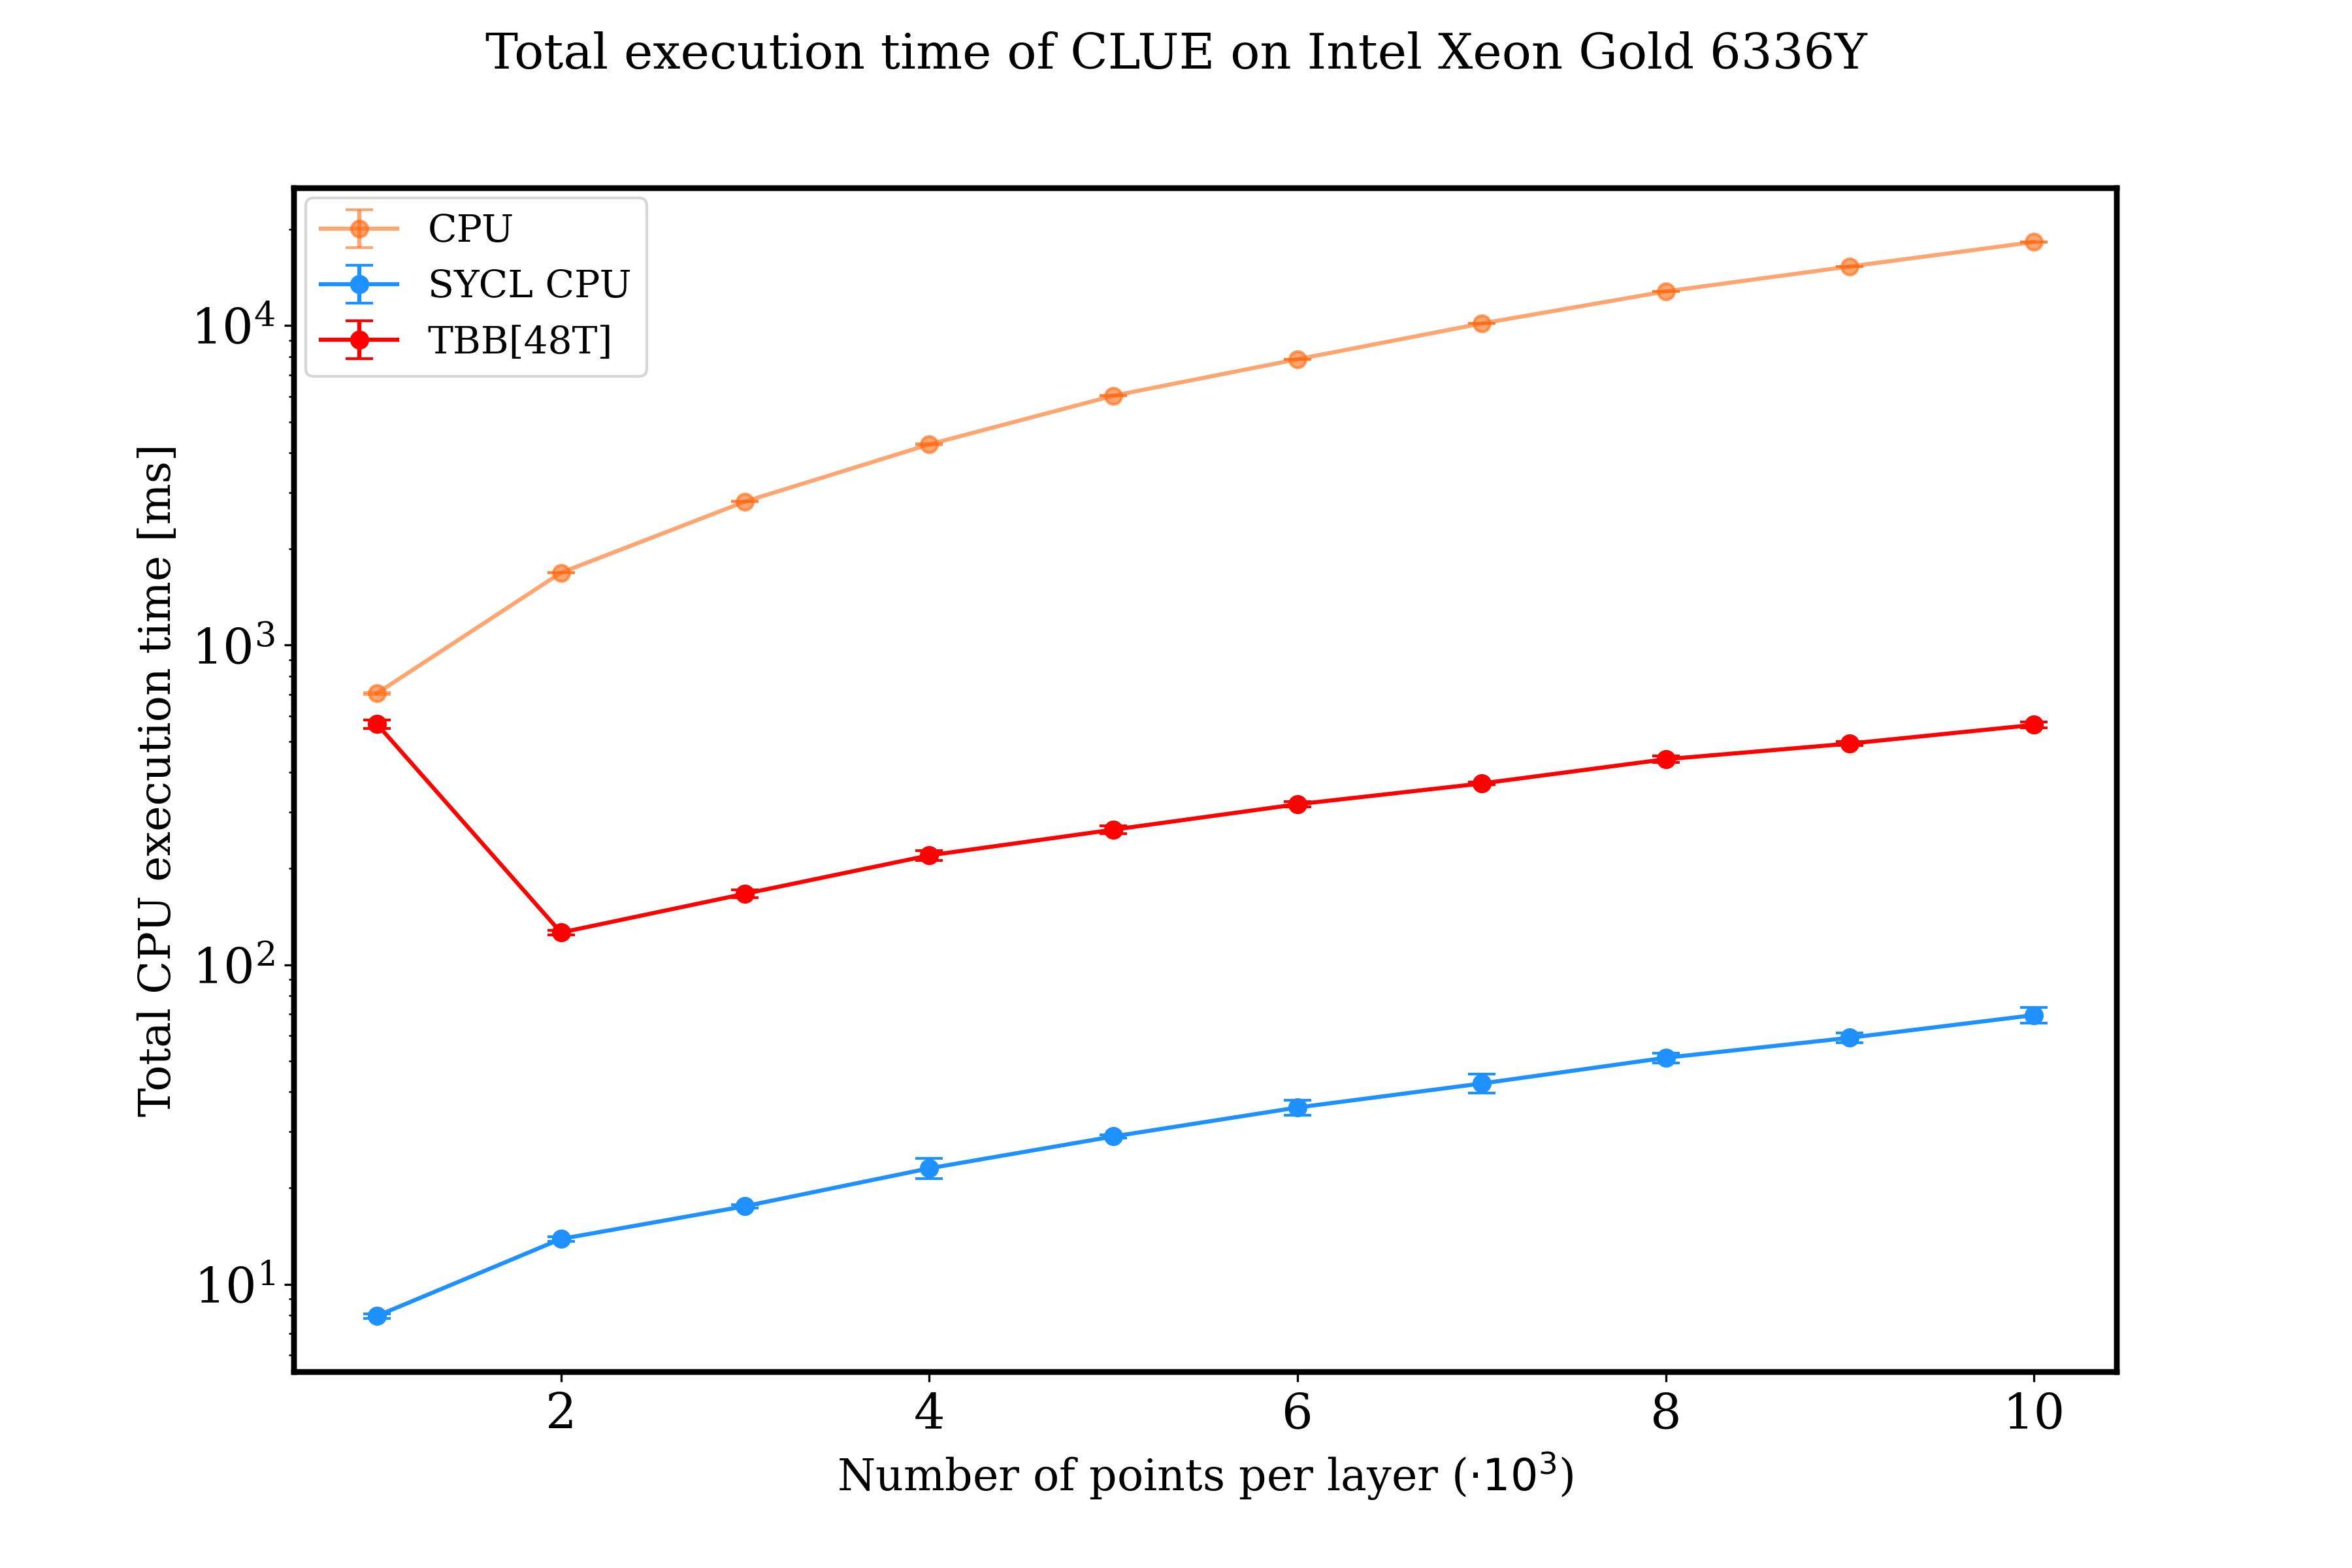
\includegraphics[width=\textwidth]{media/clue_standalone_cpu.png}
    \caption{Performance comparison of CLUE's different CPU implementations (lower execution time is better). Note that the y-axis is in log scale, showing the massive improvement that SYCL has over the native serial code. This advantage is mostly given by the native support for multi-threading in SYCL applications.}
    \label{fig:clue_standalone_cpu}
\end{figure}

The largest speedup factor in execution time is achieved by using GPUs. The main aim of the porting was to show that it is possible to write a single source code to compile and run on a multitude of devices. In Figure~\ref{fig:clue_standalone_cuda} it is shown how the total execution time of CLUE running on the same GPU is similar when using SYCL with the CUDA backend and native CUDA code. SYCL code is completely unchanged compared to the CPU version shown above, thus achieving at least one of the objectives of using portability layers in heterogeneous computing scenarios. The only difference between this executable and the one used for the CPU benchmark is the compiler that produced it. In fact, oneAPI's compiler, \texttt{dpcpp}, does not yet support the CUDA backend natively and is still in development; therefore, an open source fork of \texttt{dpcpp}, \texttt{LLVM}, was used to compile the project and test it on NVIDIA hardware. The results look extremely promising, especially considering that this backend is not officially supported yet.

\begin{figure}[H]
    \centering
    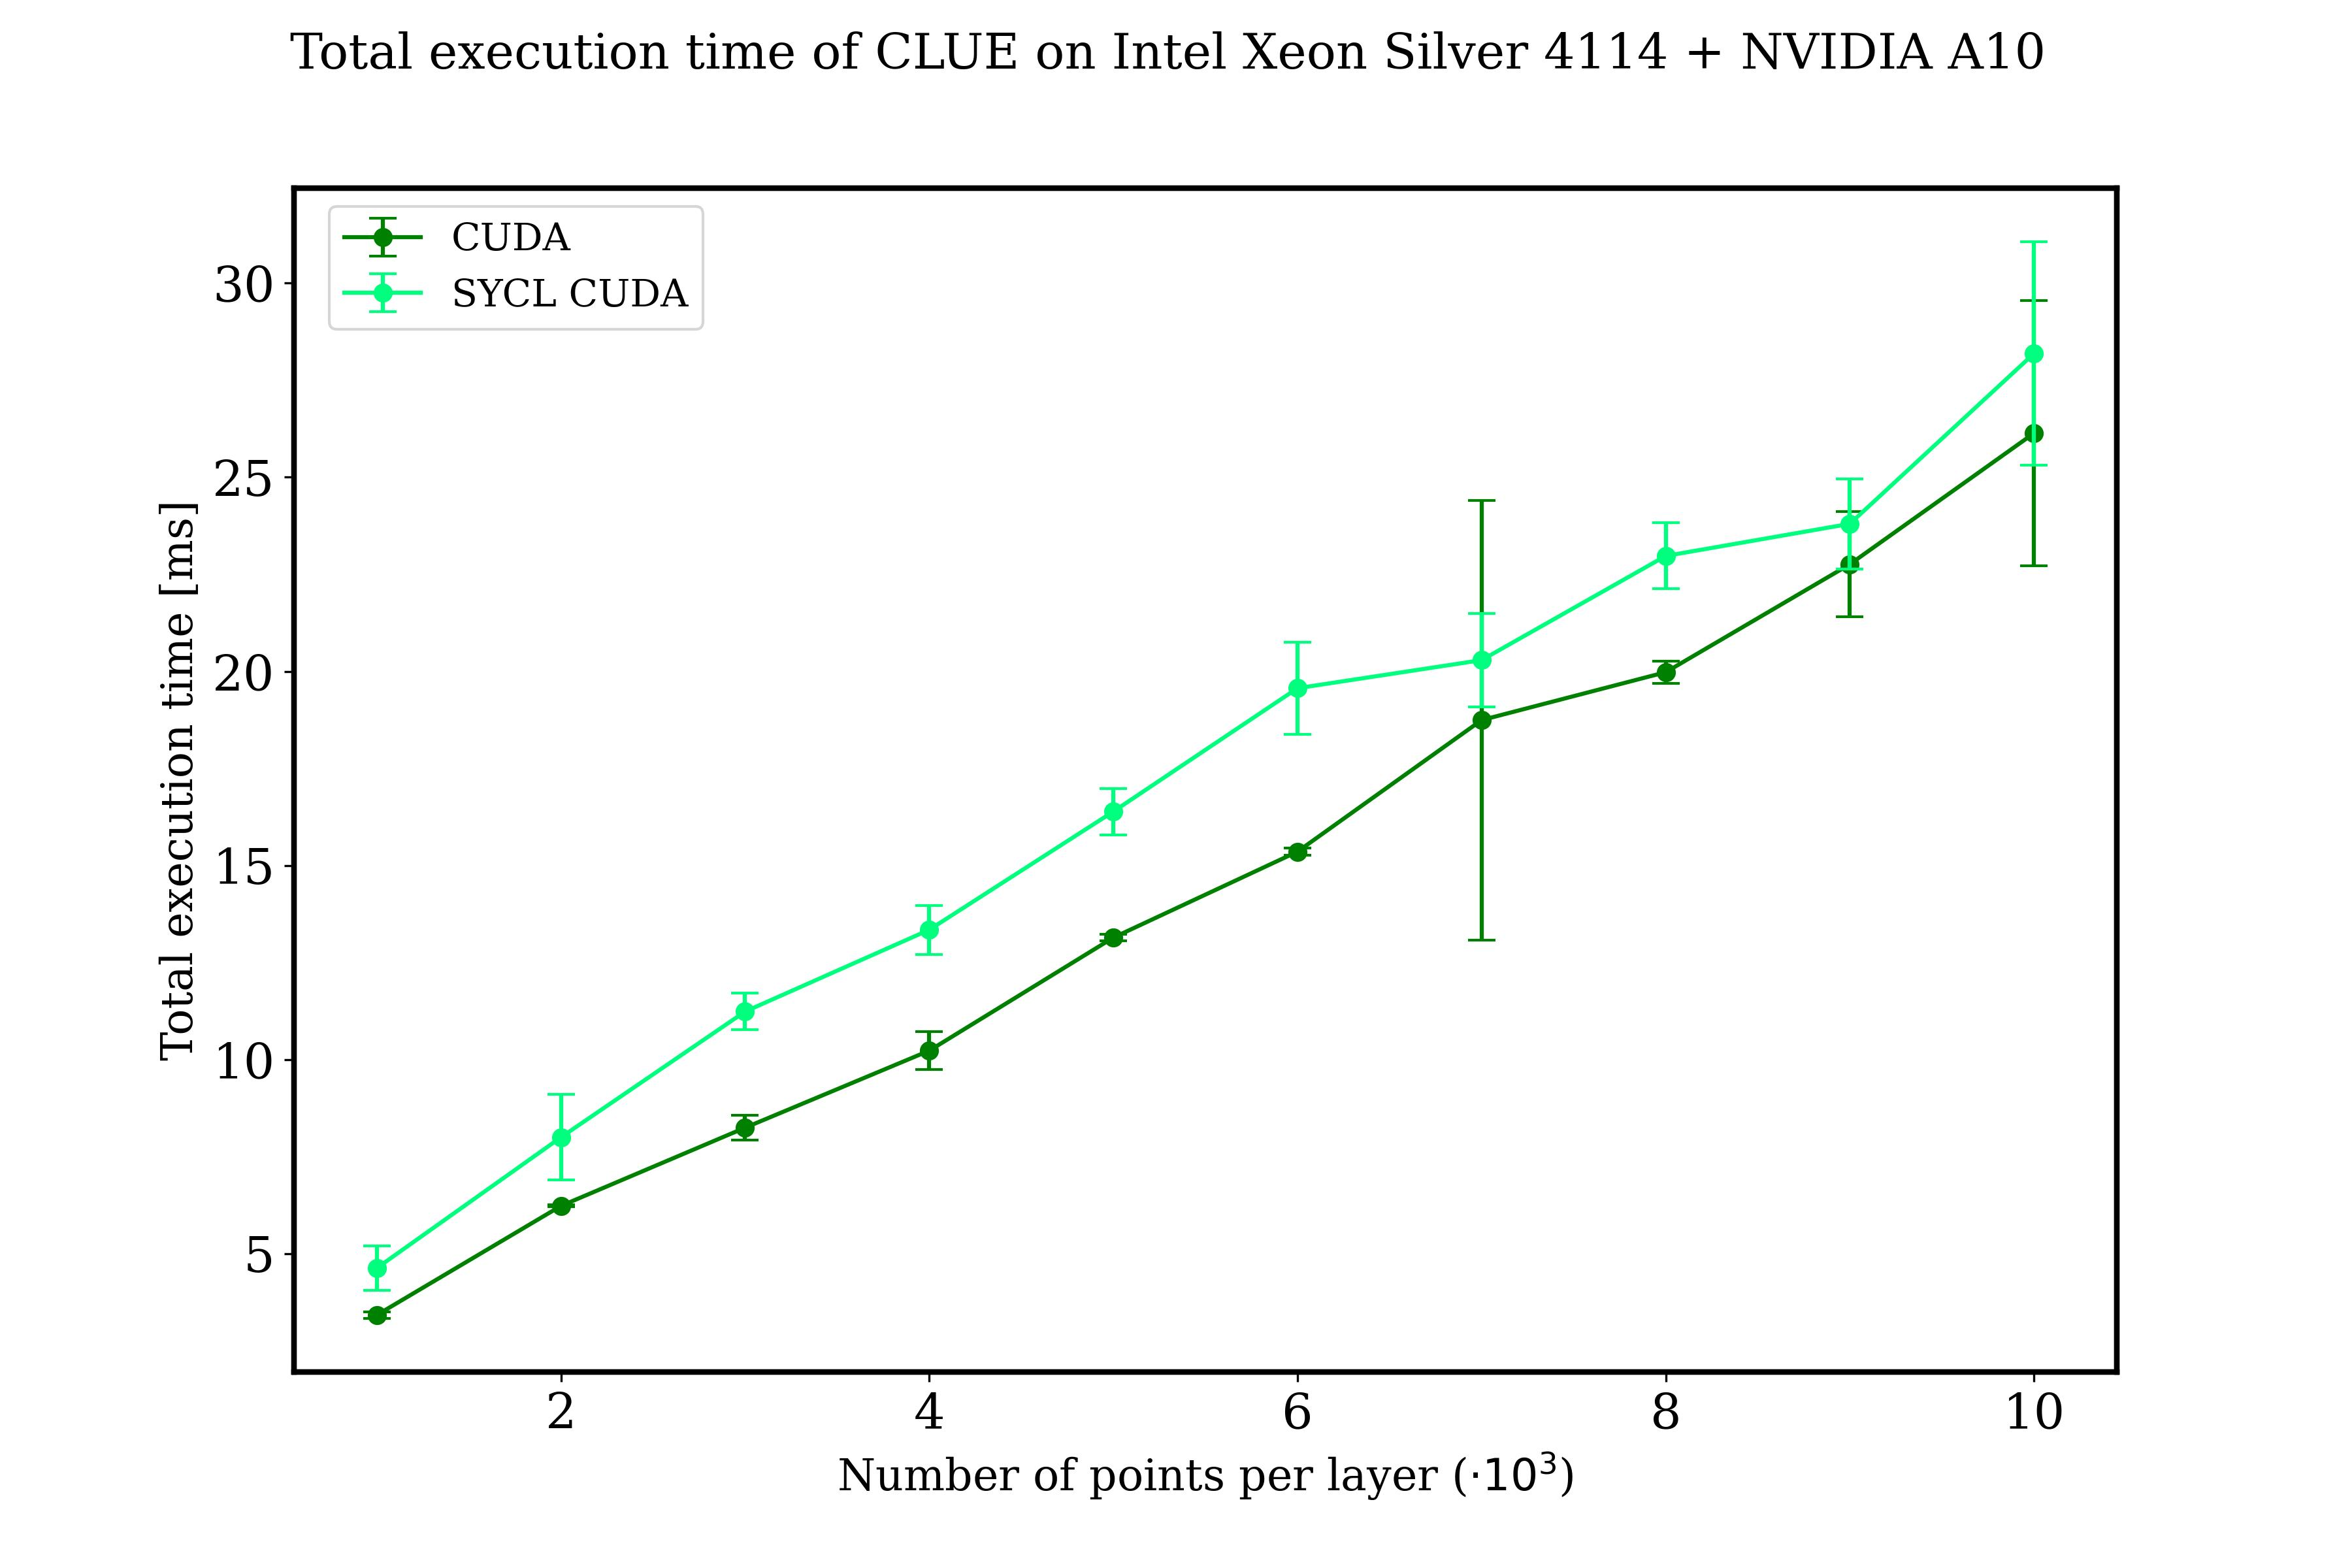
\includegraphics[width=\textwidth]{media/clue_standalone_cuda.jpg}
    \caption{Performance comparison between native CUDA code and SYCL code running through the CUDA backend (lower execution time is better).}
    \label{fig:clue_standalone_cuda}
\end{figure}

Note that, in general, using GPUs allows to improve the performance by roughly a factor 3, when compared to the multi-threaded execution on CPU, and even more when considering the other implementations.

\section{Integrating CLUE in a CMSSW-like framework}
The porting of the standalone version of CLUE was carried out mainly to experiment with SYCL and become familiar with its functioning. Once the task was completed, actual physics evaluation and performance measurements had to be carried out in a framework resembling the one used in CMSSW. Although this required significant changes and adaptations as well as actual developments on the framework itself,  better results were obtained in terms of both raw performance and physics reconstruction.

\subsection{An introduction to the framework}
Similarly to what has previously been done by the Patatrack CMS group for the standalone pixel track and vertex reconstruction~\cite{pixeltrack}, an approximation of CMSSW framework~\cite{cmssw} was used to process data and schedule the execution of CLUE, from now on referred to as heterogeneous CLUE. 

The main goal of the framework is to facilitate the deployment of software and test both already-consolidated and new algorithms in a realistic testbed before including them in the official software of the CMS experiment. The core of the execution is the Event Data Model (EDM) which is centered around the concept of \emph{Event}. Topologically, an Event is a C++ object which contains all the raw data and information related to simultaneous collisions whose average number is known as pileup and which form a single particle collision event. In the specific case of CLUE, each Event contains the 2D coordinates, layer, and energy of every hit produced by a collision event. The Event is used to pass data from one module to the next and it represents the only way to access or modify data. Some modules might require additional information to process events that are provided through the \emph{Event Setup} module. Furthermore, the framework is modular, meaning that each step of the reconstruction is represented by a separate plugin that can be plugged into the main run. Plugins are compiled in shared libraries and the execution must be configured to schedule and run the desired plugins. Although the framework includes six different types of modules, only the following ones are used with the CLUE algorithm:
\begin{itemize}
    \item Source: Produces one or more Events by reading data from an input file (csv, binary, ROOT...), gives the Event status information, and can add data on host memory. 
    \item EDProducer: Producer modules read data from an Event, produce an outcome and put it back into the Event.
    \item OutputModule: Reads data from the Event and stores the output to external media.
\end{itemize}

In this context, it is possible to offload part of the workload to accelerators when using one of the implementations of the framework and modules that take advantage of a compatibility layer such as Alpaka or SYCL.

Figure~\ref{fig:hclue_workflow} shows heterogeneous CLUE's workflow step by step. Modules are grouped by color and the arrows indicate the order of execution. The red module is an under development integration of the 3D clustering module used in CMSSW reconstruction. Each producer module can have an associated ESProducer, used to add relevant information to the Event through the Event Setup, like the parameters needed for clustering. 

\begin{figure}[H]
    \centering
    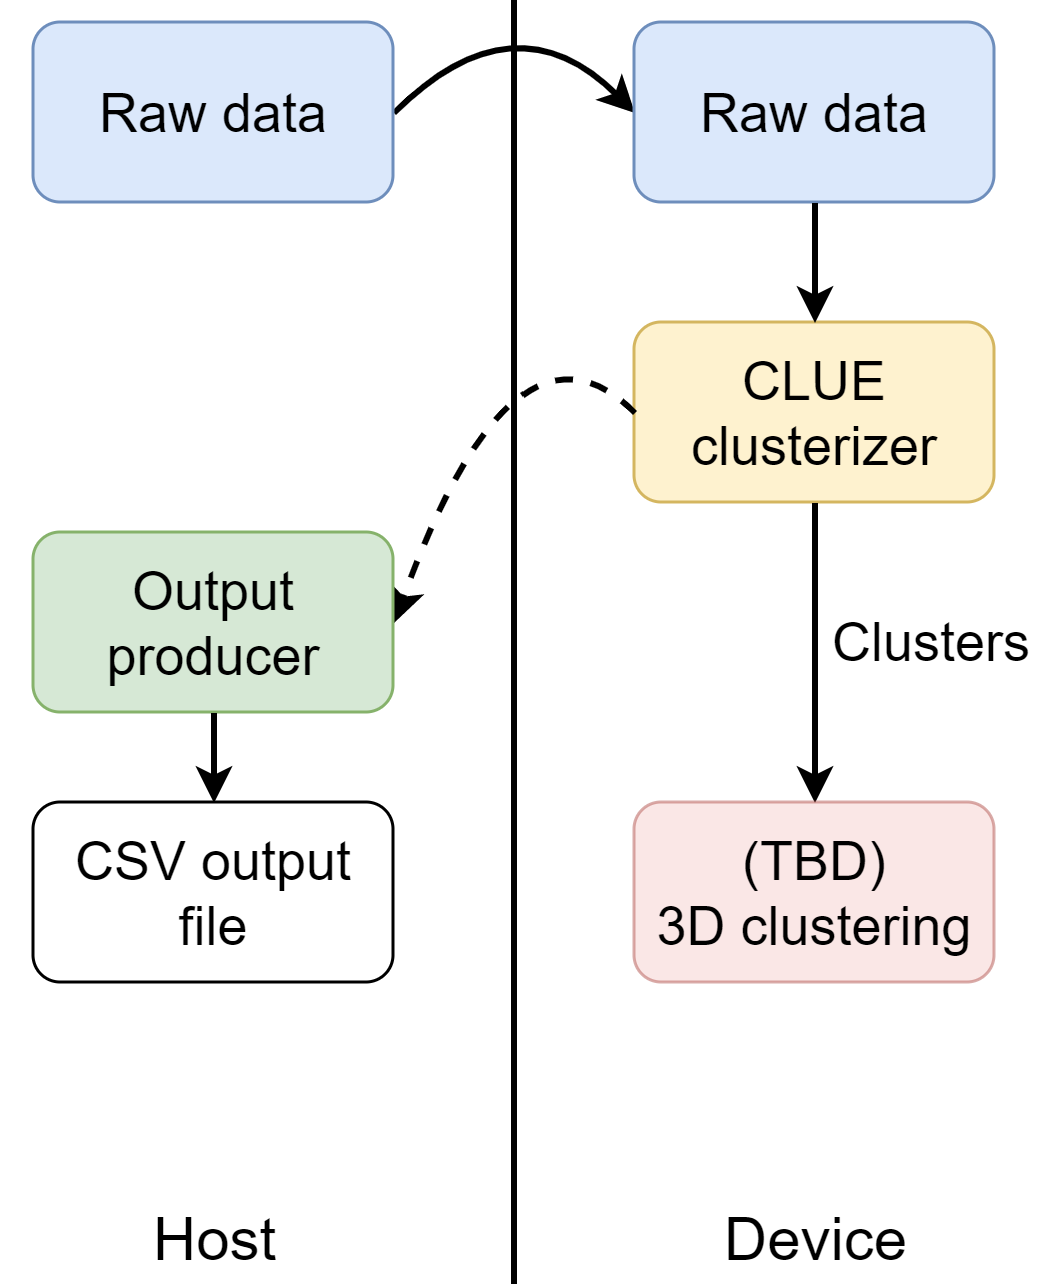
\includegraphics[scale=0.7]{media/hclue_workflow.png}
    \caption{Heterogeneous CLUE workflow. Blue modules are the results of Source, the yellow module is the single EDProducer, while the green module is the OutputModule which (optionally) produces a csv output file per event at the end.}
    \label{fig:hclue_workflow}
\end{figure}

Another fundamental aspect of the framework is its integration with Threading Building Blocks to take advantage of multiple threads and process more events at the same time. This last aspect, in particular, is carried out by creating multiple \texttt{EDM streams}. Each of them executes the entire workflow (except for the Source, reads data from all the events only once per run) on a different event and the framework allows the creation and execution of multiple streams at the same time. This means that on a more capable device, like a multi-threaded CPU or a GPU, multiple events can be analyzed at the same time, thus greatly increasing the total throughput achieved by the algorithm.
CLUE hence acts as a somewhat simple introduction to the framework's inner workings and provides a benchmarking platform for the different implementations. It is important to note that detaching modules from CMSSW and integrating them into standalone versions of the framework allows to experiment new algorithms, data structures and memory management methods as well as to test performance without having to interface them with the full reconstruction of the CMS detector. Such idea of a testbed has led to the creation to the standalone pixel tracking module as well as this CLUE implementation.

\subsection{Changes and improvements from the standalone version}
Integrating CLUE in the framework allows taking advantage of more efficient scheduling, and finer control of the number of threads and concurrent streams used for the execution while also providing better performance measuring capabilities. However, in order to fully take advantage of the framework, significant changes had to be made to the core of its SYCL implementation. 

Starting from the most fundamental aspect, some parts of the framework, ported from CUDA, needed to be optimized for SYCL's inner workings, while some others had to be rewritten entirely. Since SYCL is designed to be compatible with multiple backends, its logic for device selection cannot match the one implemented in CUDA and is rather similar to alpaka. In the current version of the code, the user can select which device to offload work to by a simple command line parameter \texttt{--device} followed by the type of device wanted or its backend. The device selector will take care of finding all of the compatible devices and offload work to the selected one by creating an in-order queue on that device per \texttt{EDM stream} to schedule memory operations and kernel execution.

When offloading work to an accelerator, the most costly operation in terms of overhead is device memory allocation. That is why the framework includes a module for caching the allocations, which had to be entirely rewritten for SYCL. This module ensures that the least amount of allocations is performed and that memory that has been freed can be reused without needing another allocation. Using CLUE as an example, the algorithm needs 13 allocations per run for input variables, results, and some inner variables used to make calculations. Using the caching allocator, when running with a single stream, CLUE will allocate 13 blocks of the required size in the device memory, then reuse those blocks for each event and finally free the device memory at the end of the execution. At the beginning of the execution one caching allocator is constructed on each available device. Device memory is accessed through custom-defined unique pointers which interface directly with the caching allocator on the specific device. This approach has two main benefits:
\begin{itemize}
    \item Costly device memory allocations are reduced to a minimum number by reusing memory whenever possible;
    \item All of the cached memory is freed at the end of the execution, thus allowing no memory leaks.
\end{itemize}

From the algorithm's point of view, these changes mainly reflect in what modules of the workflow are allowed to allocate device memory. Since a single \texttt{sycl::queue} is produced per event and gets propagated by the framework and considering that the queue is needed for all of the memory operations and kernels scheduling, the algorithm needed some optimizations to perform queue-bound operations only when one is obtainable from the \texttt{EDM event}.

\section{Results}
Heterogeneous CLUE, was tested with a simulated dataset obtained by running the reconstruction of a $t\bar{t}$ event with 200 pileup on a recent version of CMMSW and dumping the information of hits to a binary file. The conditions chosen are the most similar to the ones that would be seen in the proposed HGCAL upgrade~\cite{hgcal}. 
\newline
In Figure~\ref{fig:whole_detector} and Figure~\ref{fig:clustering_window} are shown the clustering results of CLUE on layer 5 of the simulated dataset. In particular, Figure~\ref{fig:whole_detector} shows hits registered in the entire detector, while Figure~\ref{fig:clustering_window} focuses on a smaller window to better show the clusters built by CLUE.

\begin{figure}[ht]
    \centering
    \begin{subfigure}[t]{0.49\textwidth}
    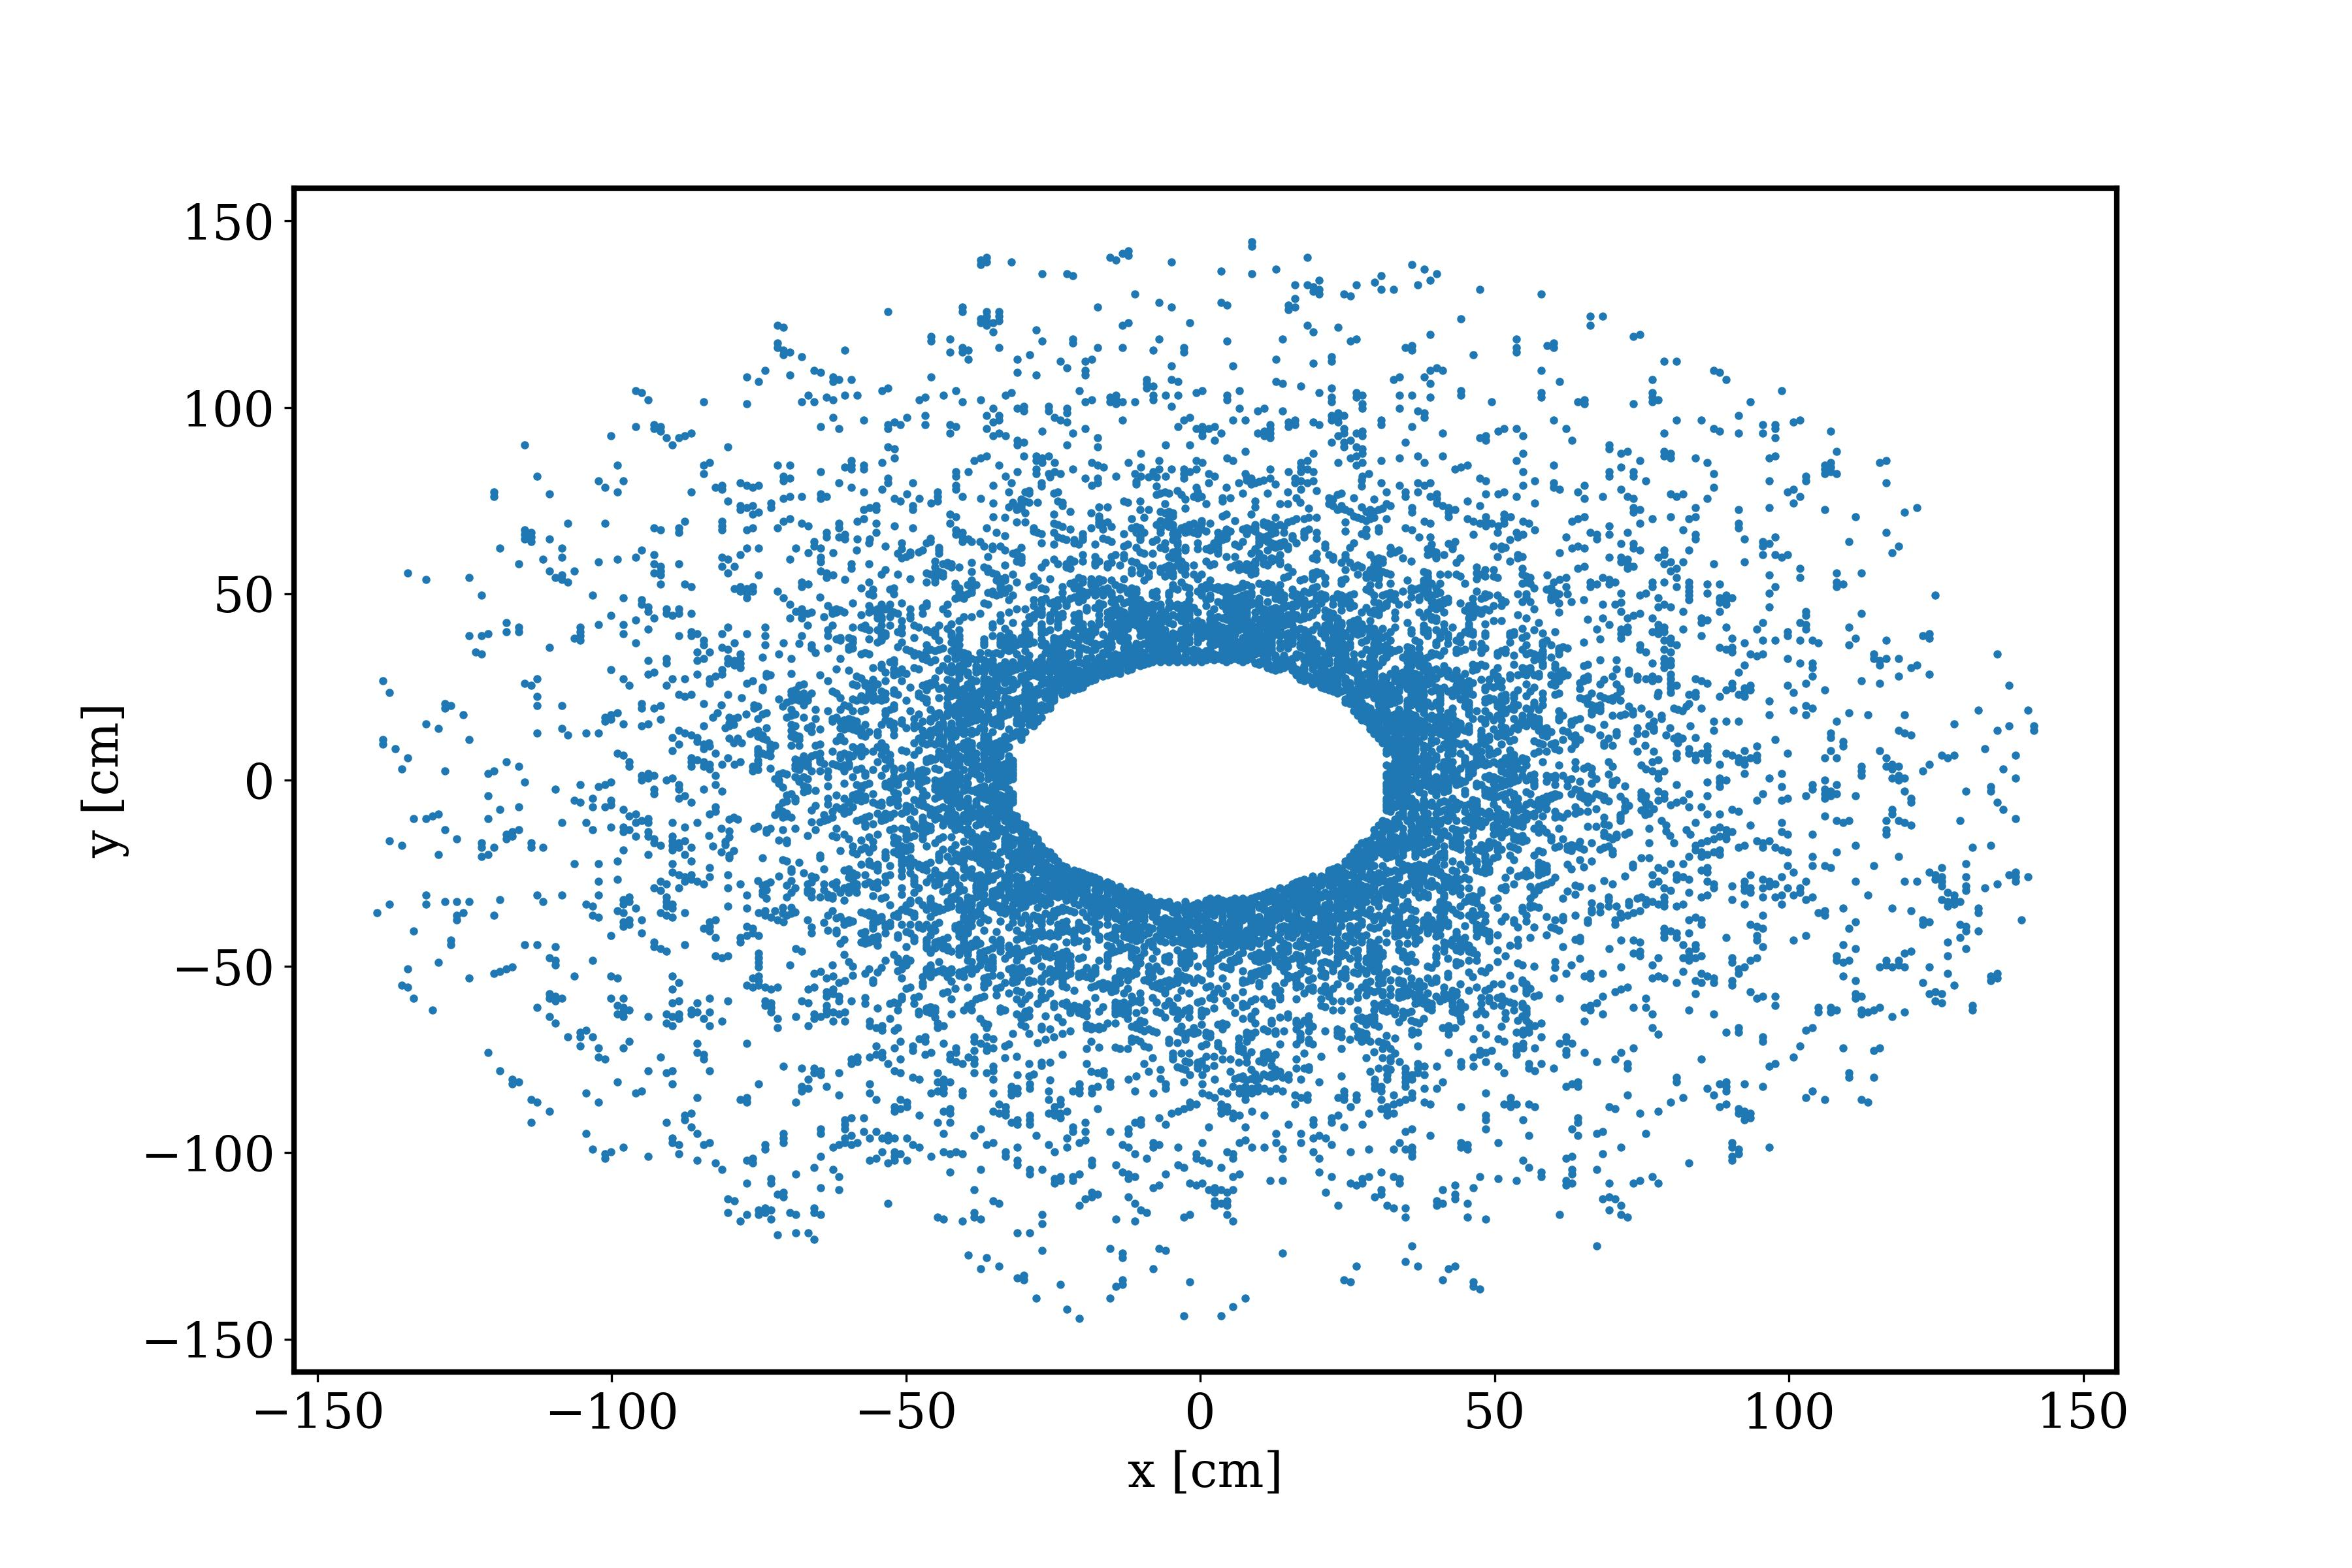
\includegraphics[width=\textwidth]{media/whole_detector.jpg}
    \caption{Input data for layer 5.}
    \end{subfigure}
    \begin{subfigure}[t]{0.49\textwidth}
    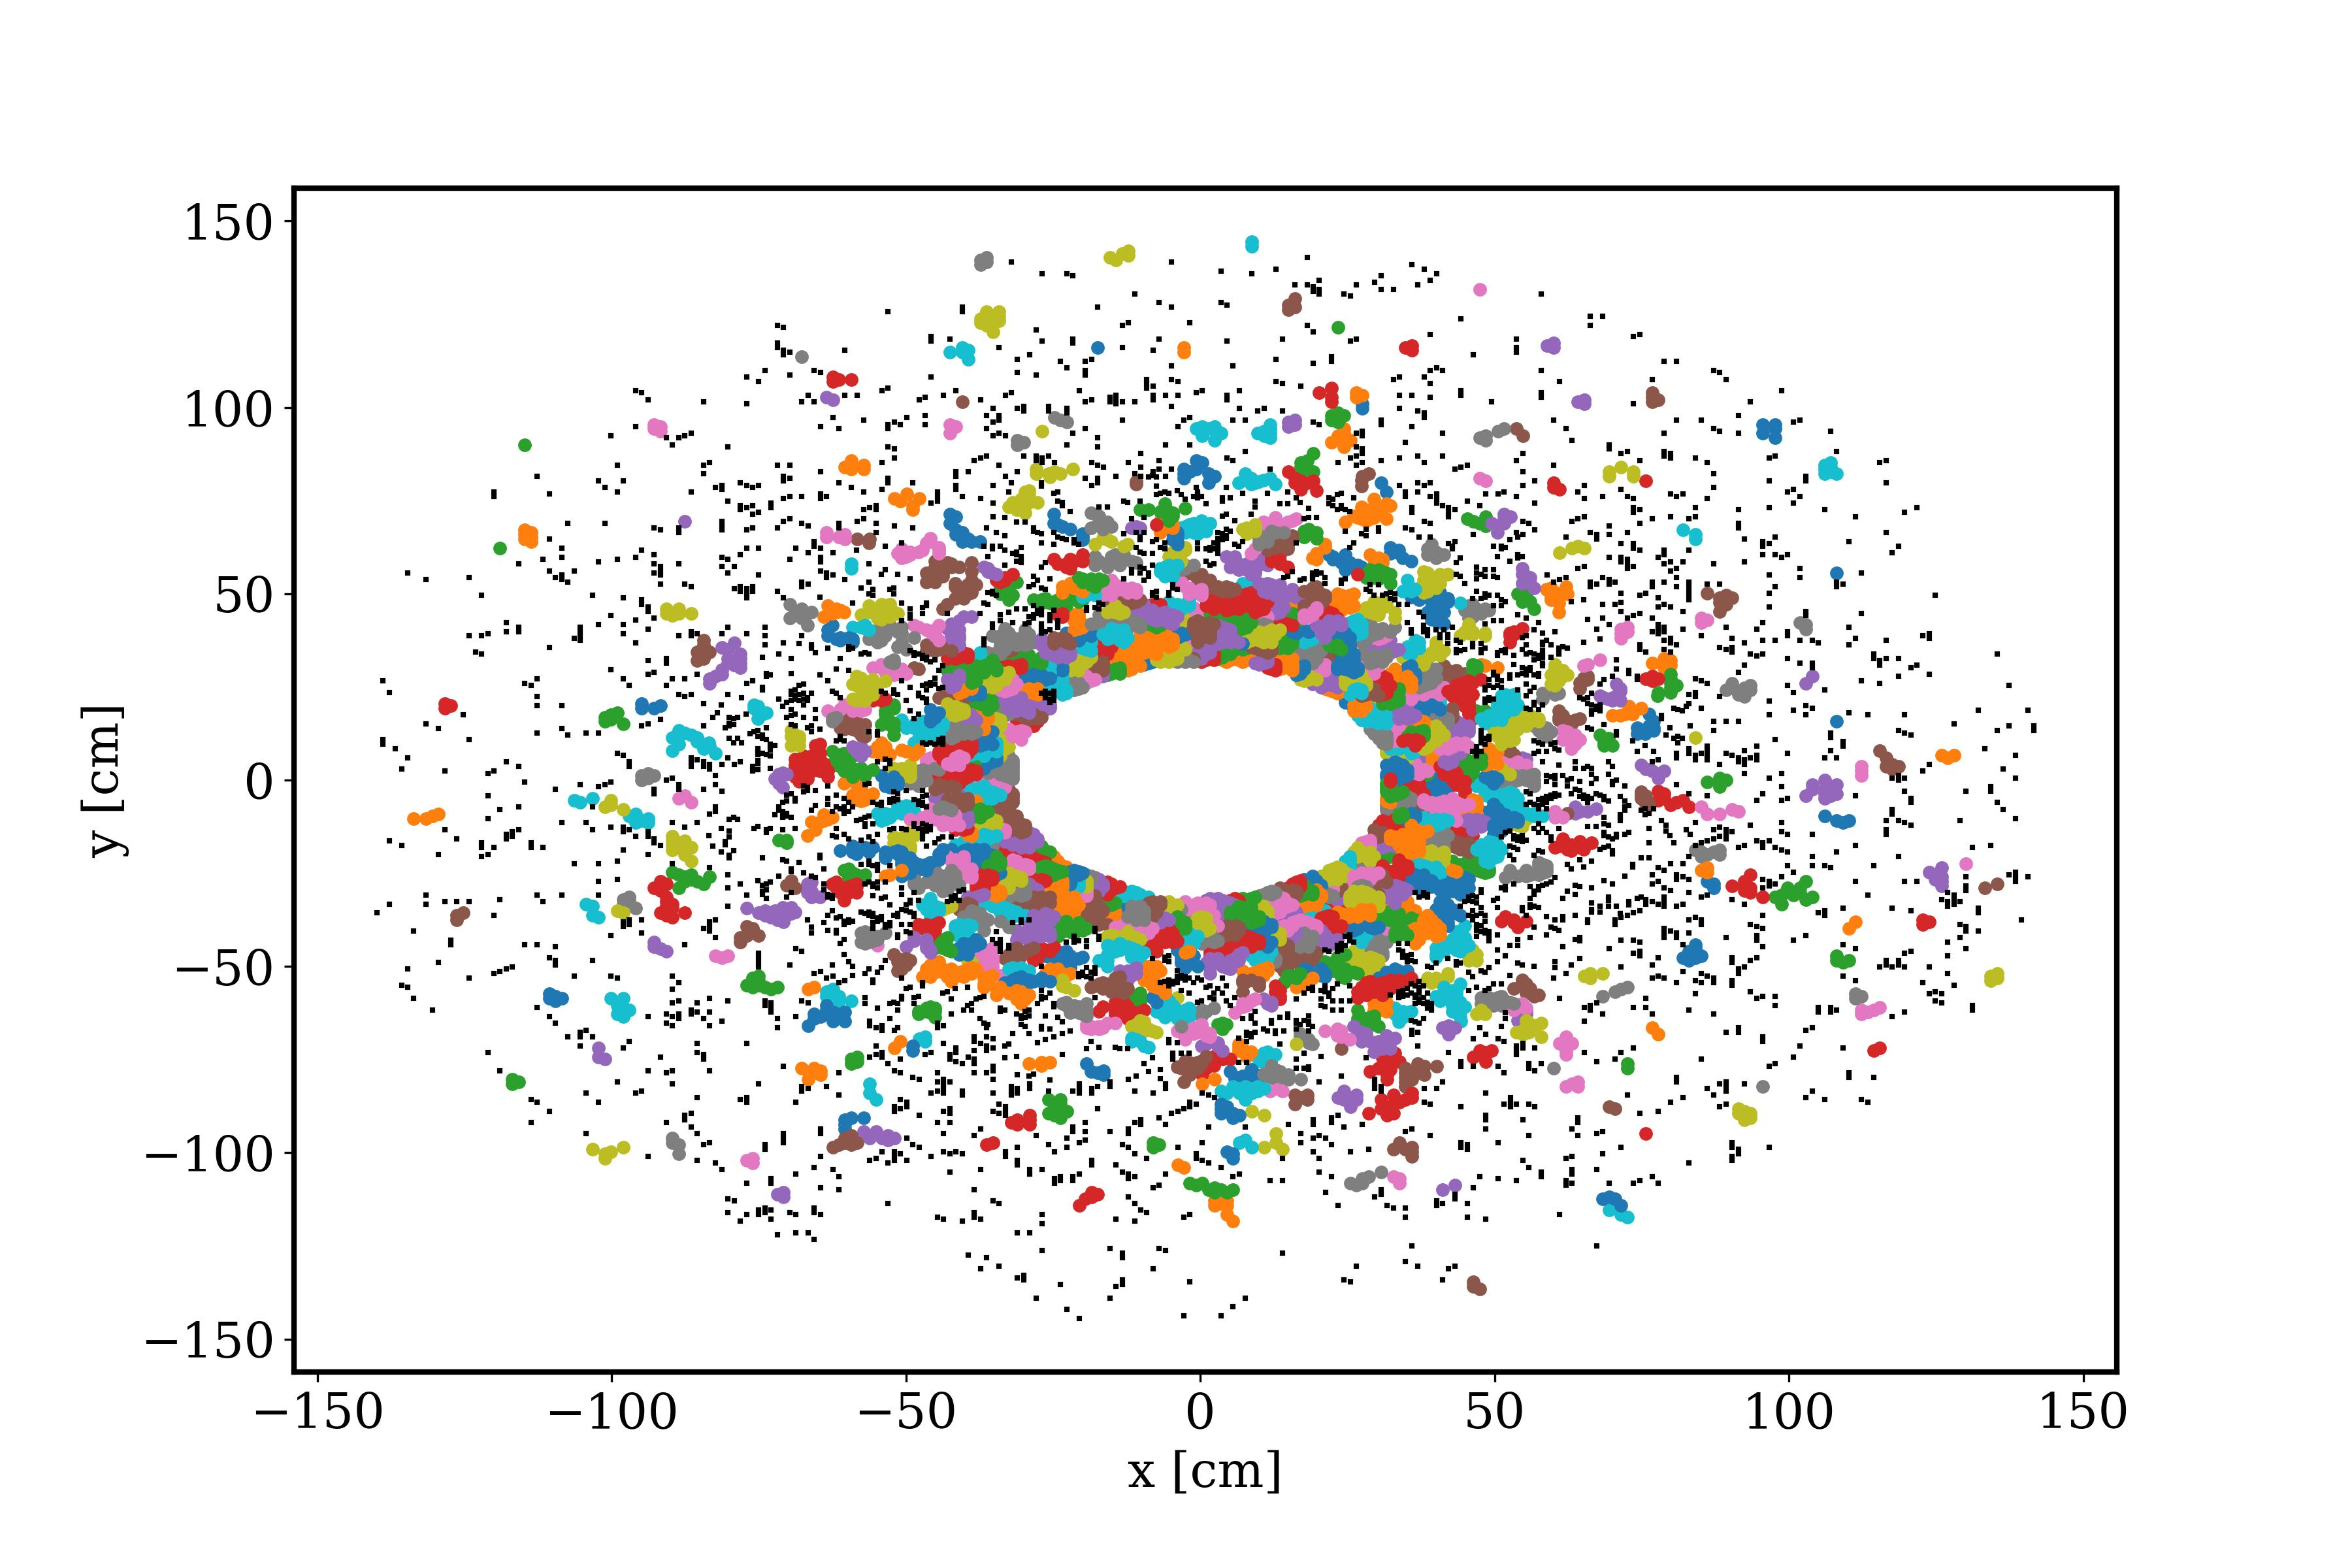
\includegraphics[width=\textwidth]{media/whole_detector_clusters.jpg}
    \caption{Clusters produced by CLUE.}
    \end{subfigure}
    \caption{Example of CLUE clustering on layer 5 of the simulated dataset dumped from CMSSW. Each cluster is characterized by a different color (with some repetitions due to the large number of clusters) while outliers are represented as black squares.}
    \label{fig:whole_detector}
\end{figure}

\begin{figure}[H]
    \centering
    \begin{subfigure}[t]{0.49\textwidth}
    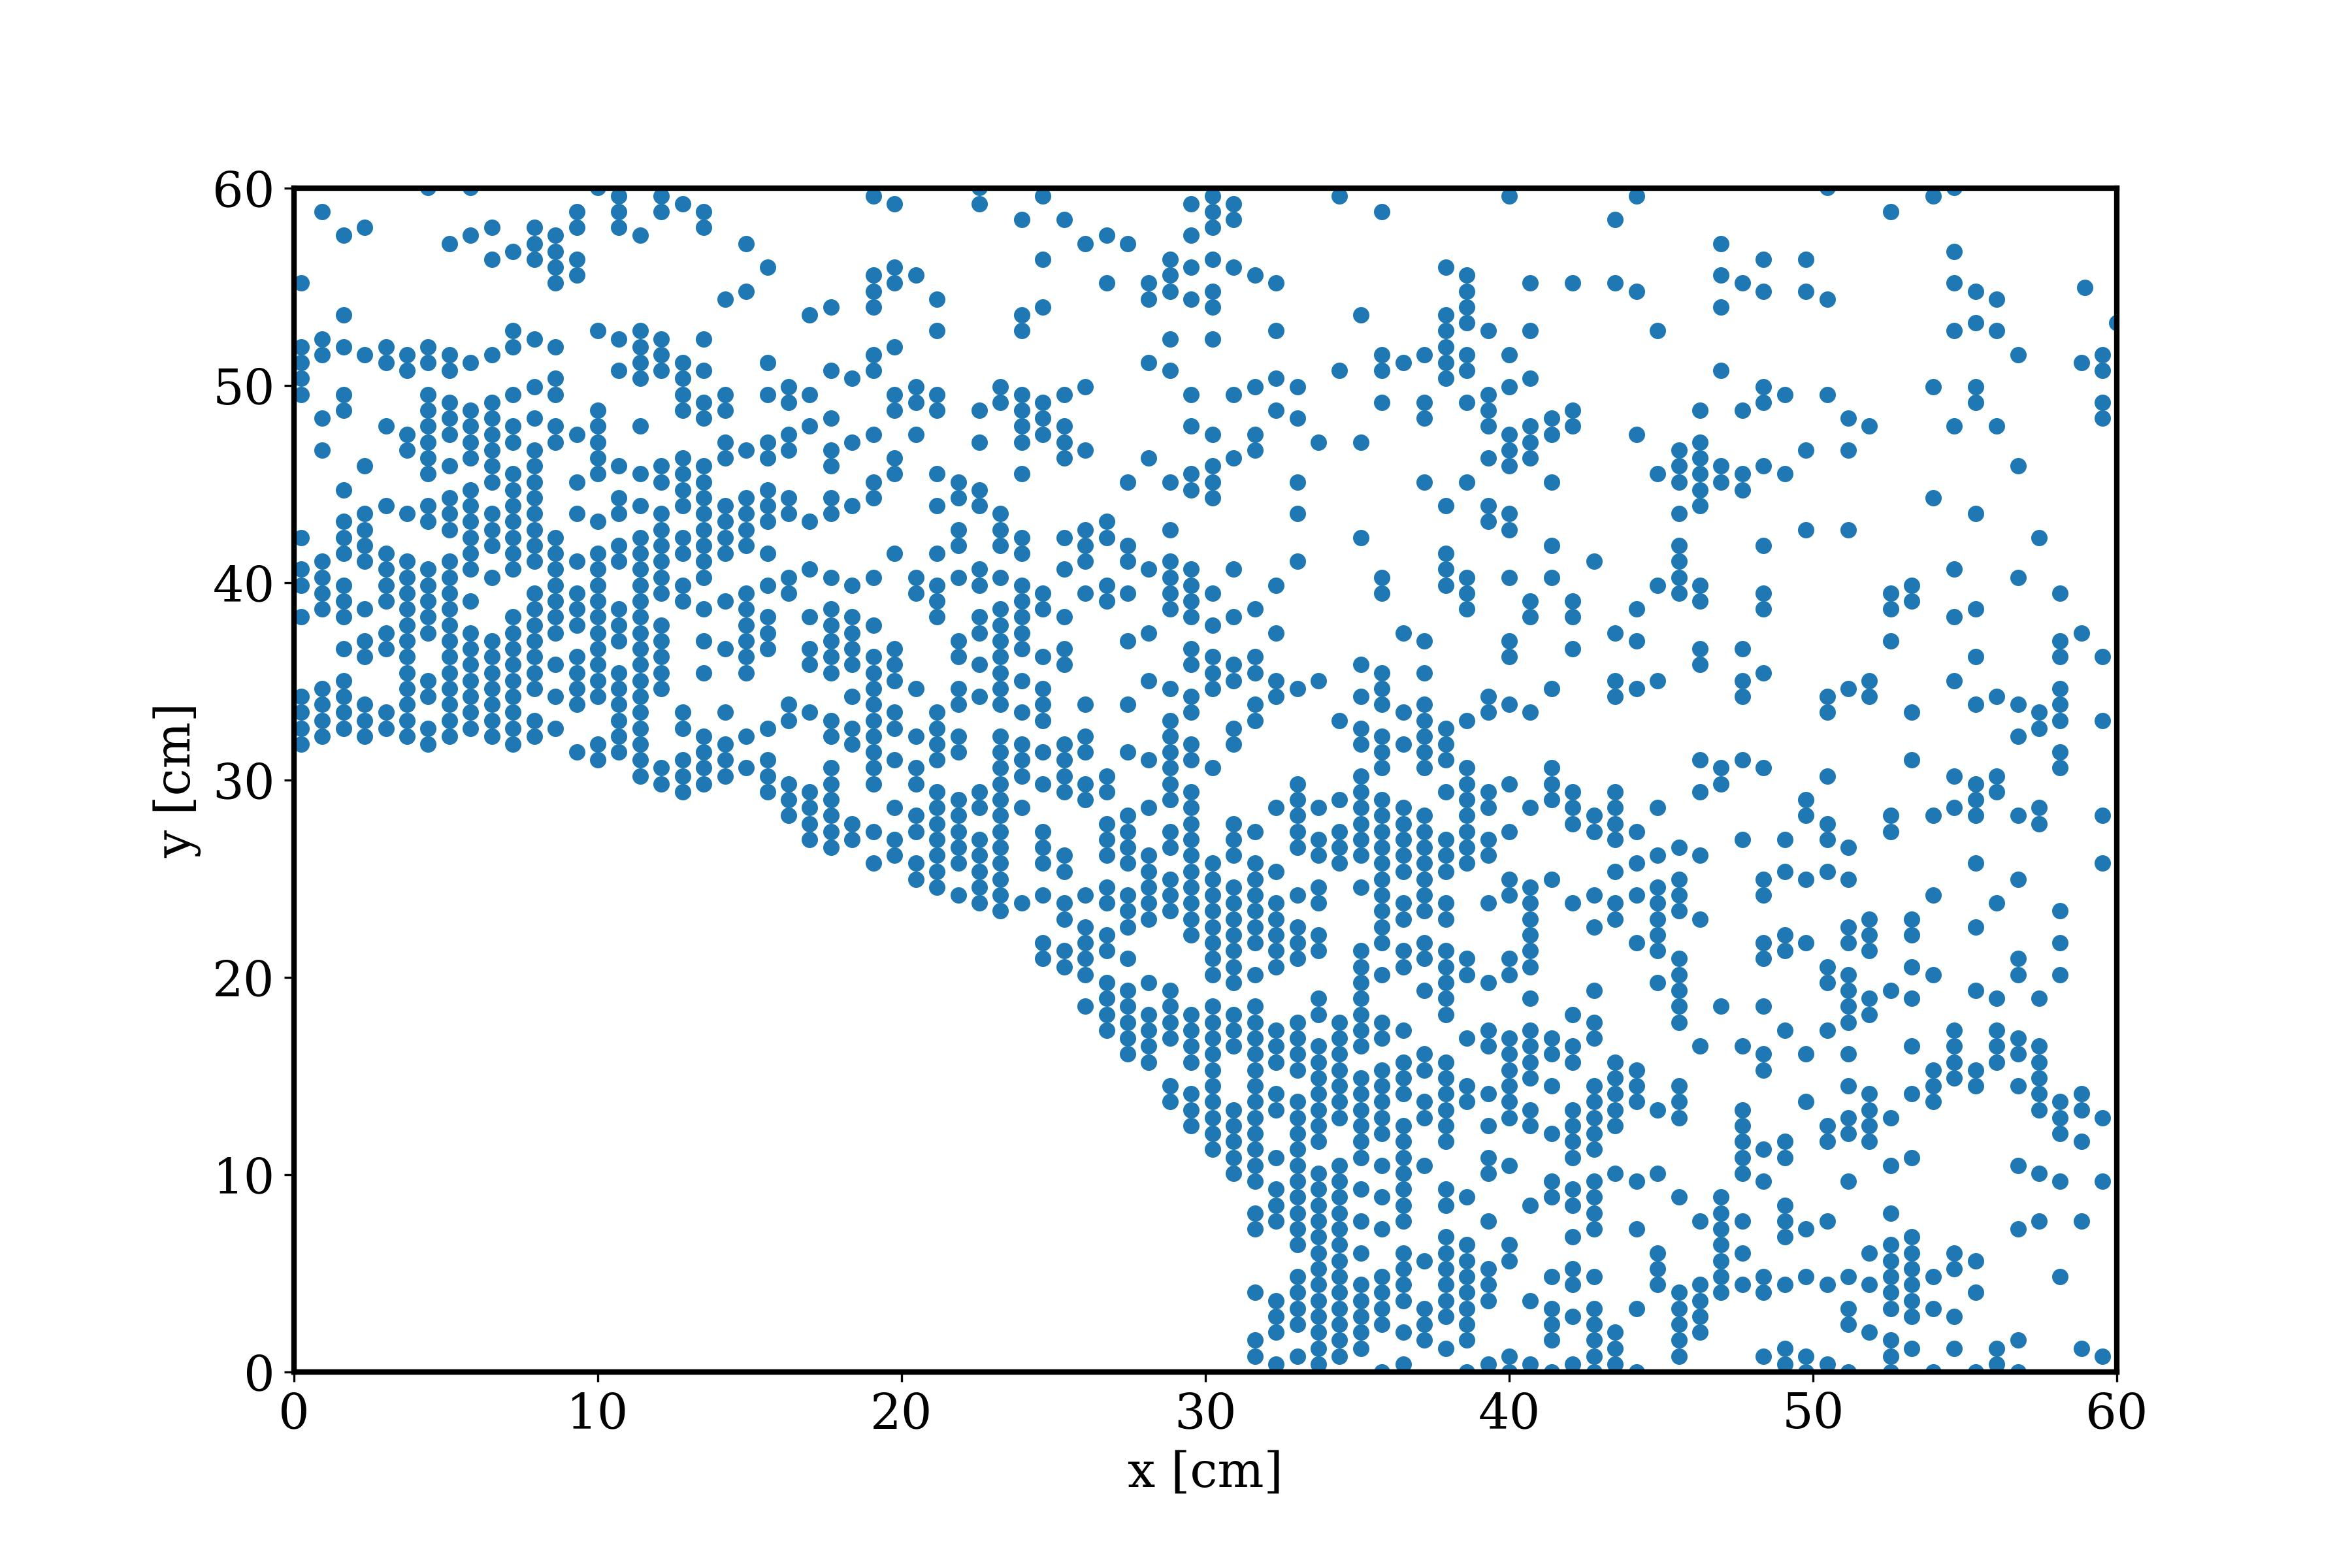
\includegraphics[width=\textwidth]{media/detector_window.jpg}
    \caption{Input data for a small window of the detector.}
    \end{subfigure}
    \begin{subfigure}[t]{0.49\textwidth}
    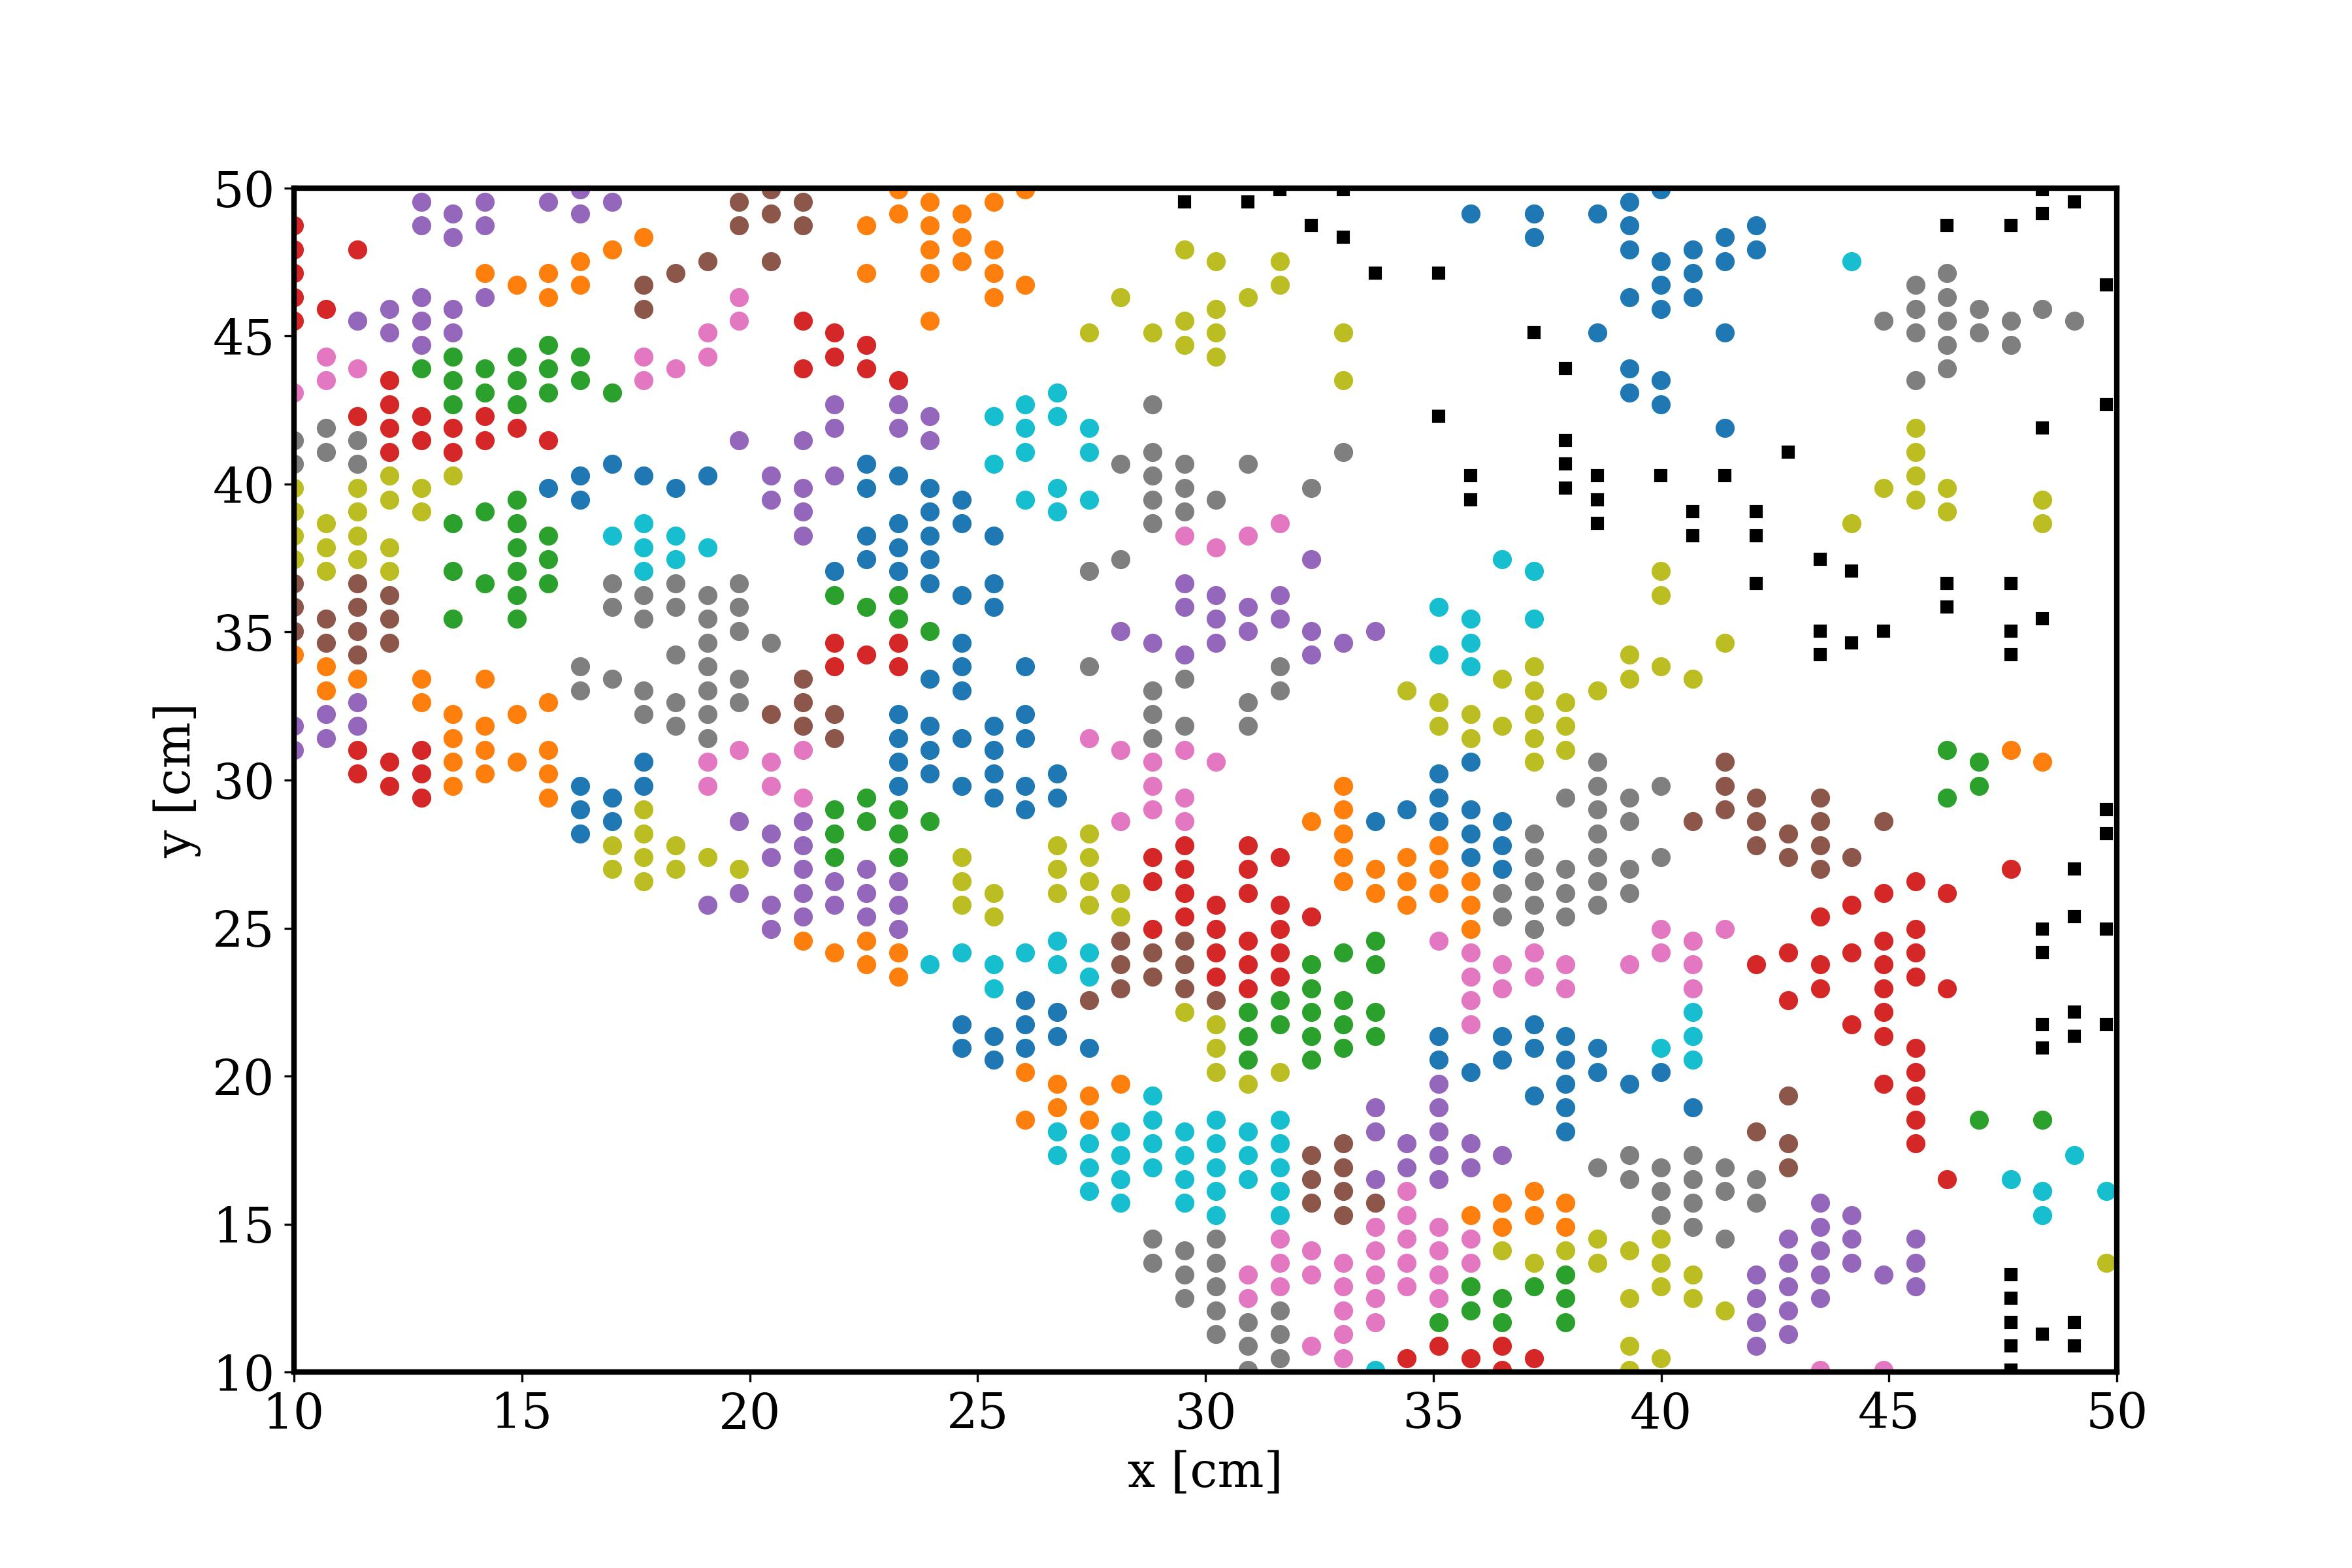
\includegraphics[width=\textwidth]{media/detector_window_clusters.jpg}
    \caption{Clusters produced by CLUE.}
    \end{subfigure}
    \caption{Clustering results of CLUE on a small detector window. Each color corresponds to a different cluster. Outliers are represented as black squares.}
    \label{fig:clustering_window}
\end{figure}

\subsection{Physics performance}
Heterogeneous CLUE's performance has been evaluated on both CPUs and GPUs with different backends using Alpaka, SYCL, and native code whenever possible. In particular, the following hardware was used to benchmark the algorithm:

\begin{itemize}
    \item Intel(R) Xeon(R) Silver 4114 CPU 2.20GHz with driver OpenCL \newline [2022.14.7.0.30\textunderscore160000];
    \item NVIDIA Tesla T4 with driver CUDA [11.6];
    \item Unreleased Intel GPU;
\end{itemize} 

Figure~\ref{fig:hclue_cpu_performance} shows the computing performance of each implementation of heterogeneous CLUE on CPU, scaling with the number of threads. As seen in the standalone version, SYCL implementation looks to be able to take better advantage of multi-threading on CPU showing a 21-57 \% performance increase when compared to Alpaka and 14-102\% improvement with respect to the native serial implementation. The measurements are obtained as the average value of 10 consecutive runs on 1000 events. The exact results are shown in Table~\ref{tab:hclue_cpu_performance}. One particular case that needs to be clarified is the single-thread execution. Both Alpaka and the native implementations show less than half the performance of SYCL in this case. This happens because SYCL is actually using two threads in this particular instance by relying on the multi-threading capabilities of the CPU and dedicating one thread to the framework execution and one to the algorithm itself. This is confirmed by observing that the throughput remains almost exactly the same when using two threads.

\begin{figure}[H]
    \centering
    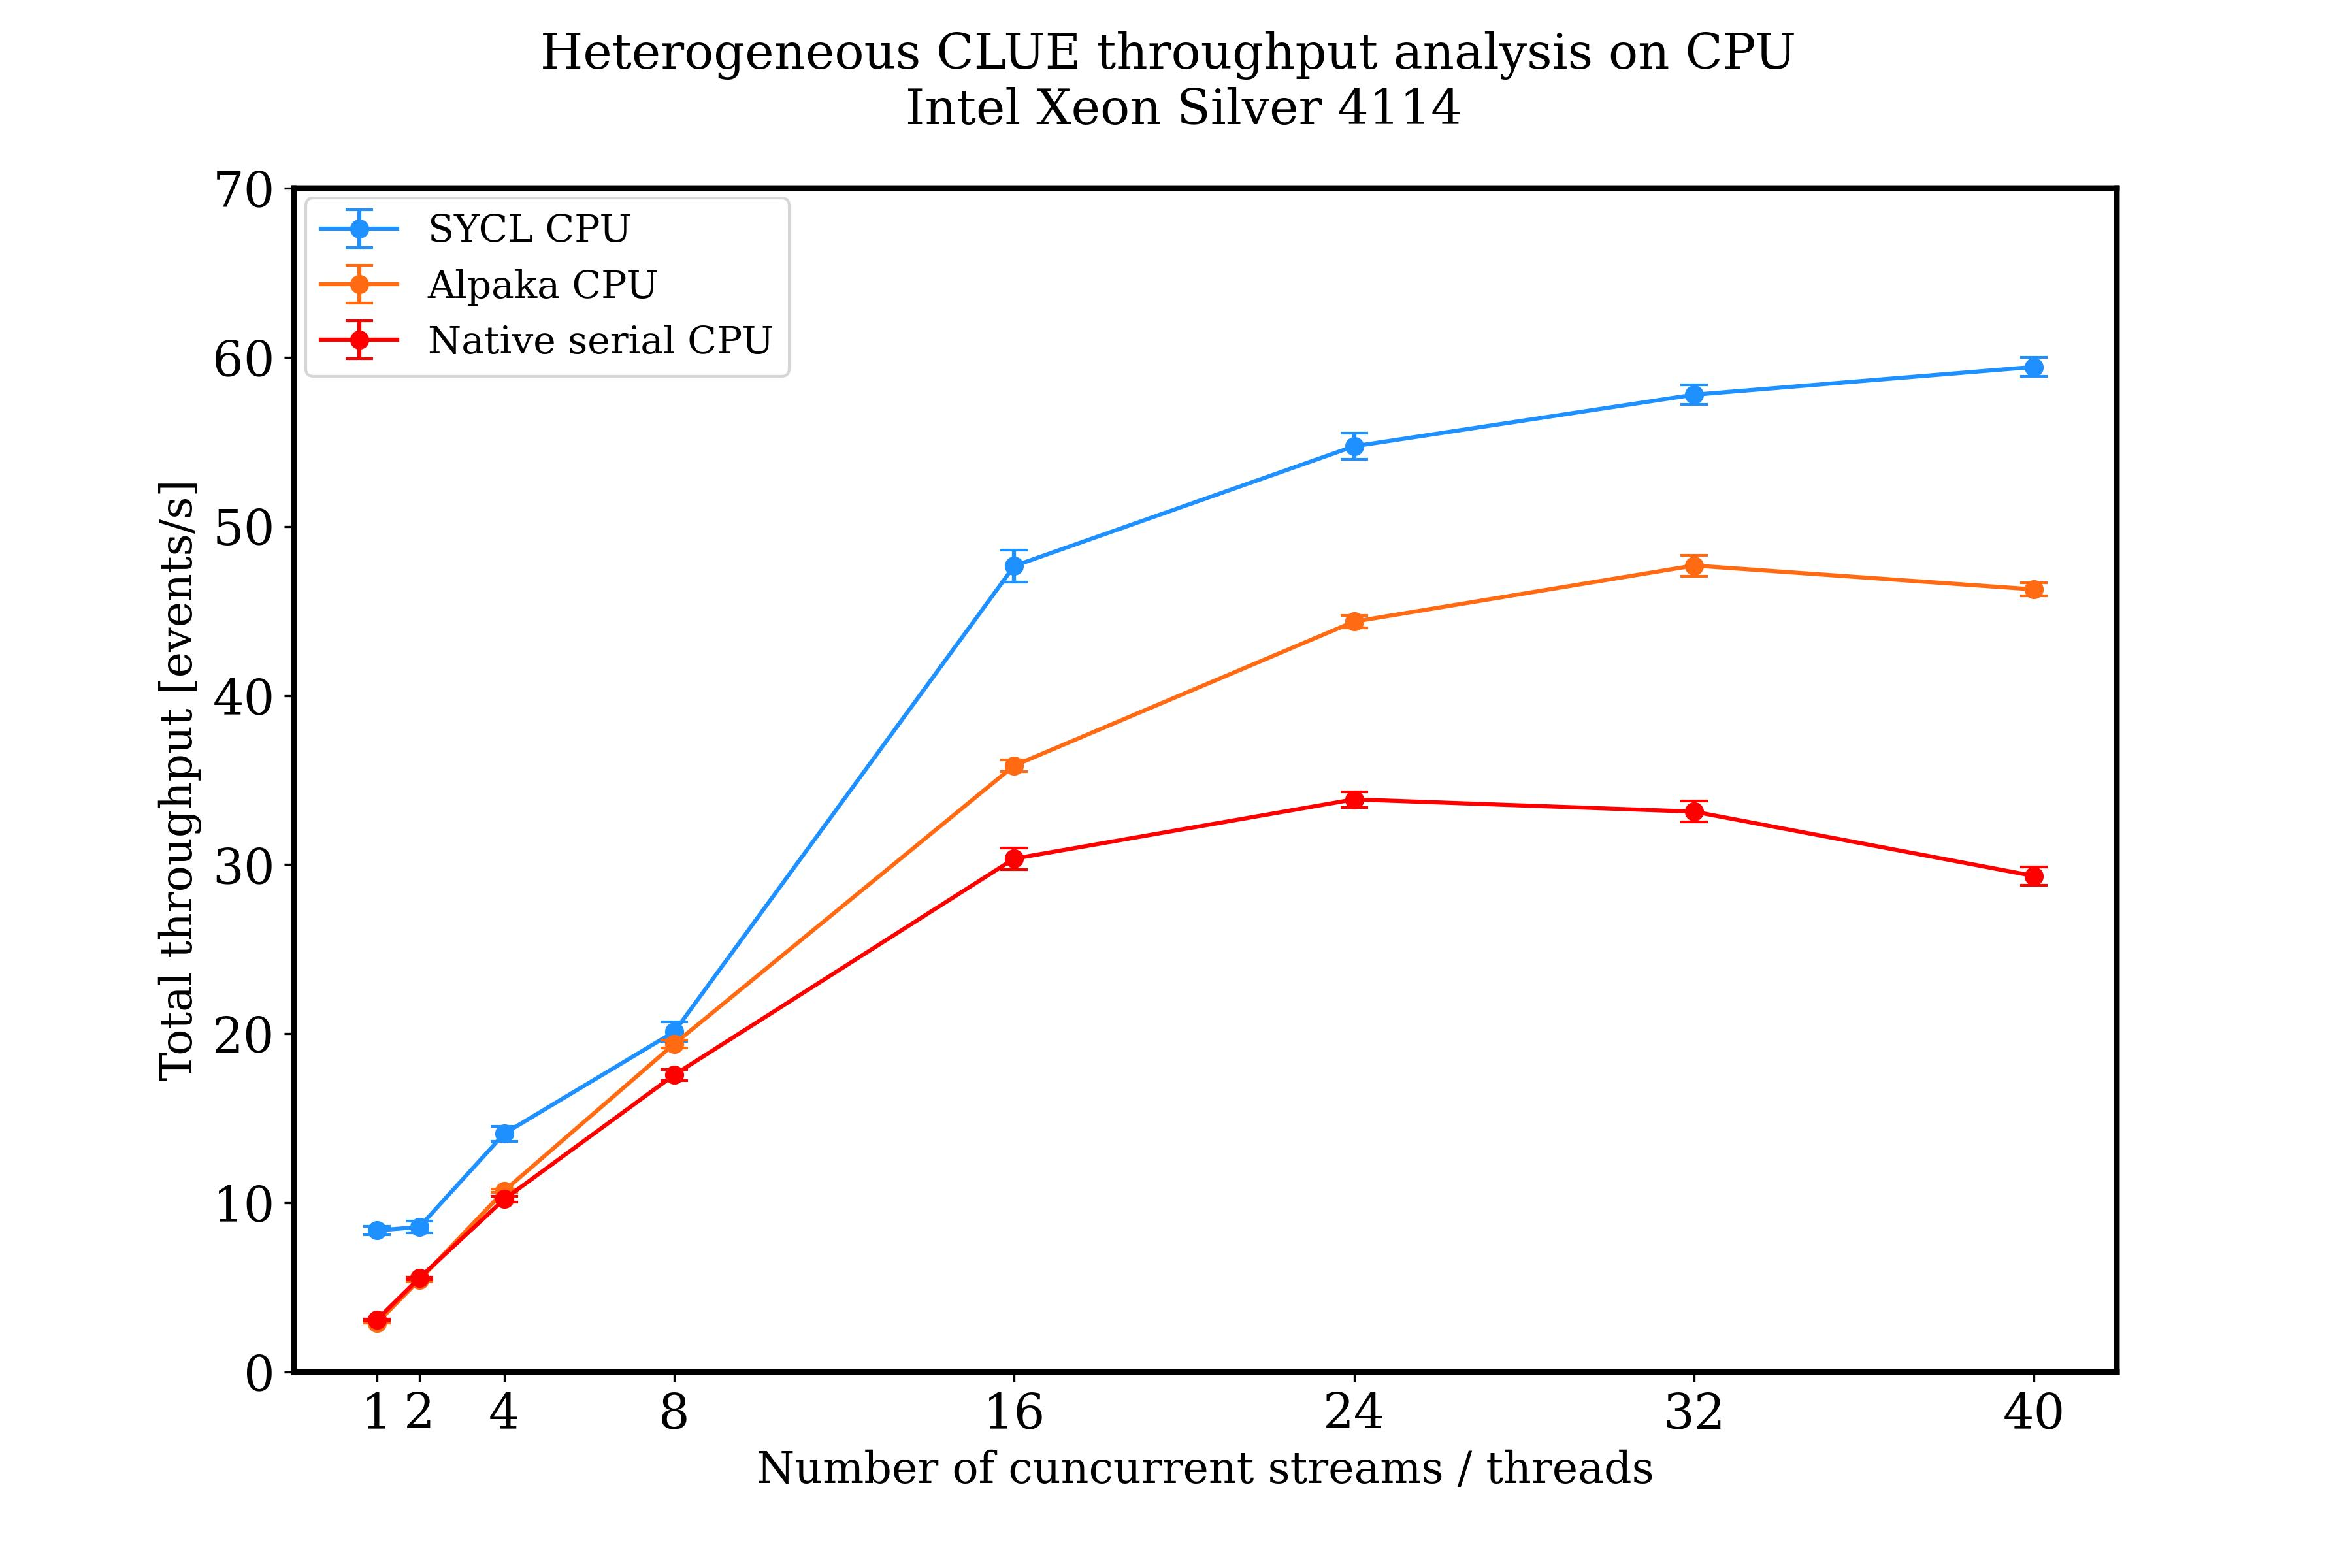
\includegraphics[width=\textwidth]{media/hclue_cpu_performance.jpg}
    \caption{Performance comparison of the different CPU implementations of heterogeneous CLUE (higher throughput is better).}
    \label{fig:hclue_cpu_performance}
\end{figure}

\begin{table}[htb]
    \centering
    \begin{tabular}{|c|r@{}c|r@{}c|r@{}c|}
 \hline
 \multicolumn{7}{|c|}{Total throughput on Intel Xeon Silver 4114 (ev/s)} \\
 \hline
 Threads & \multicolumn{2}{c|}{Alpaka} & \multicolumn{2}{c|}{Native serial} & \multicolumn{2}{c|}{SYCL}\\
 \hline
 1 & 2.894 $\pm$& ~0.014 & 3.09 $\pm$&  ~0.05 & 8.4 $\pm$&  ~0.3 \\
 2 & 5.44 $\pm$& ~0.12 & 5.55 $\pm$& ~0.05 & 8.6 $\pm$& ~0.3 \\
 4 & 10.72 $\pm$& ~0.09 &	10.22 $\pm$& ~0.15 & 14.1 $\pm$& ~0.4 \\
 8 & 19.4 $\pm$& ~0.2 & 17.6 $\pm$& ~0.3 & 20.1 $\pm$& ~0.6 \\
 16 & 35.9 $\pm$& ~0.4 & 30.4 $\pm$& ~0.6 & 47.7 $\pm$& ~0.9 \\
 24	& 44.4 $\pm$& ~0.4 & 33.9 $\pm$& ~0.5 & 54.7 $\pm$& ~0.8 \\
 32	& 47.7 $\pm$& ~0.6 & 33.1 $\pm$& ~0.6 & 57.8 $\pm$& ~0.6 \\
 40	& 46.2 $\pm$& ~0.4	& 29.3 $\pm$& ~0.5	& 59.4 $\pm$& ~0.6 \\
 \hline
\end{tabular}
    \caption{Detailed throughput analysis for the CPU implementations of heterogeneous CLUE.}
    \label{tab:hclue_cpu_performance}
\end{table}

For the GPU implementations, the throughput increases from 3 to 10 times depending on the comparisons. Figure~\ref{fig:hclue_cuda_performance} shows the comparisons between the two different compatibility layers discussed, executing logically identical code on the same hardware.

\begin{figure}[H]
    \centering
    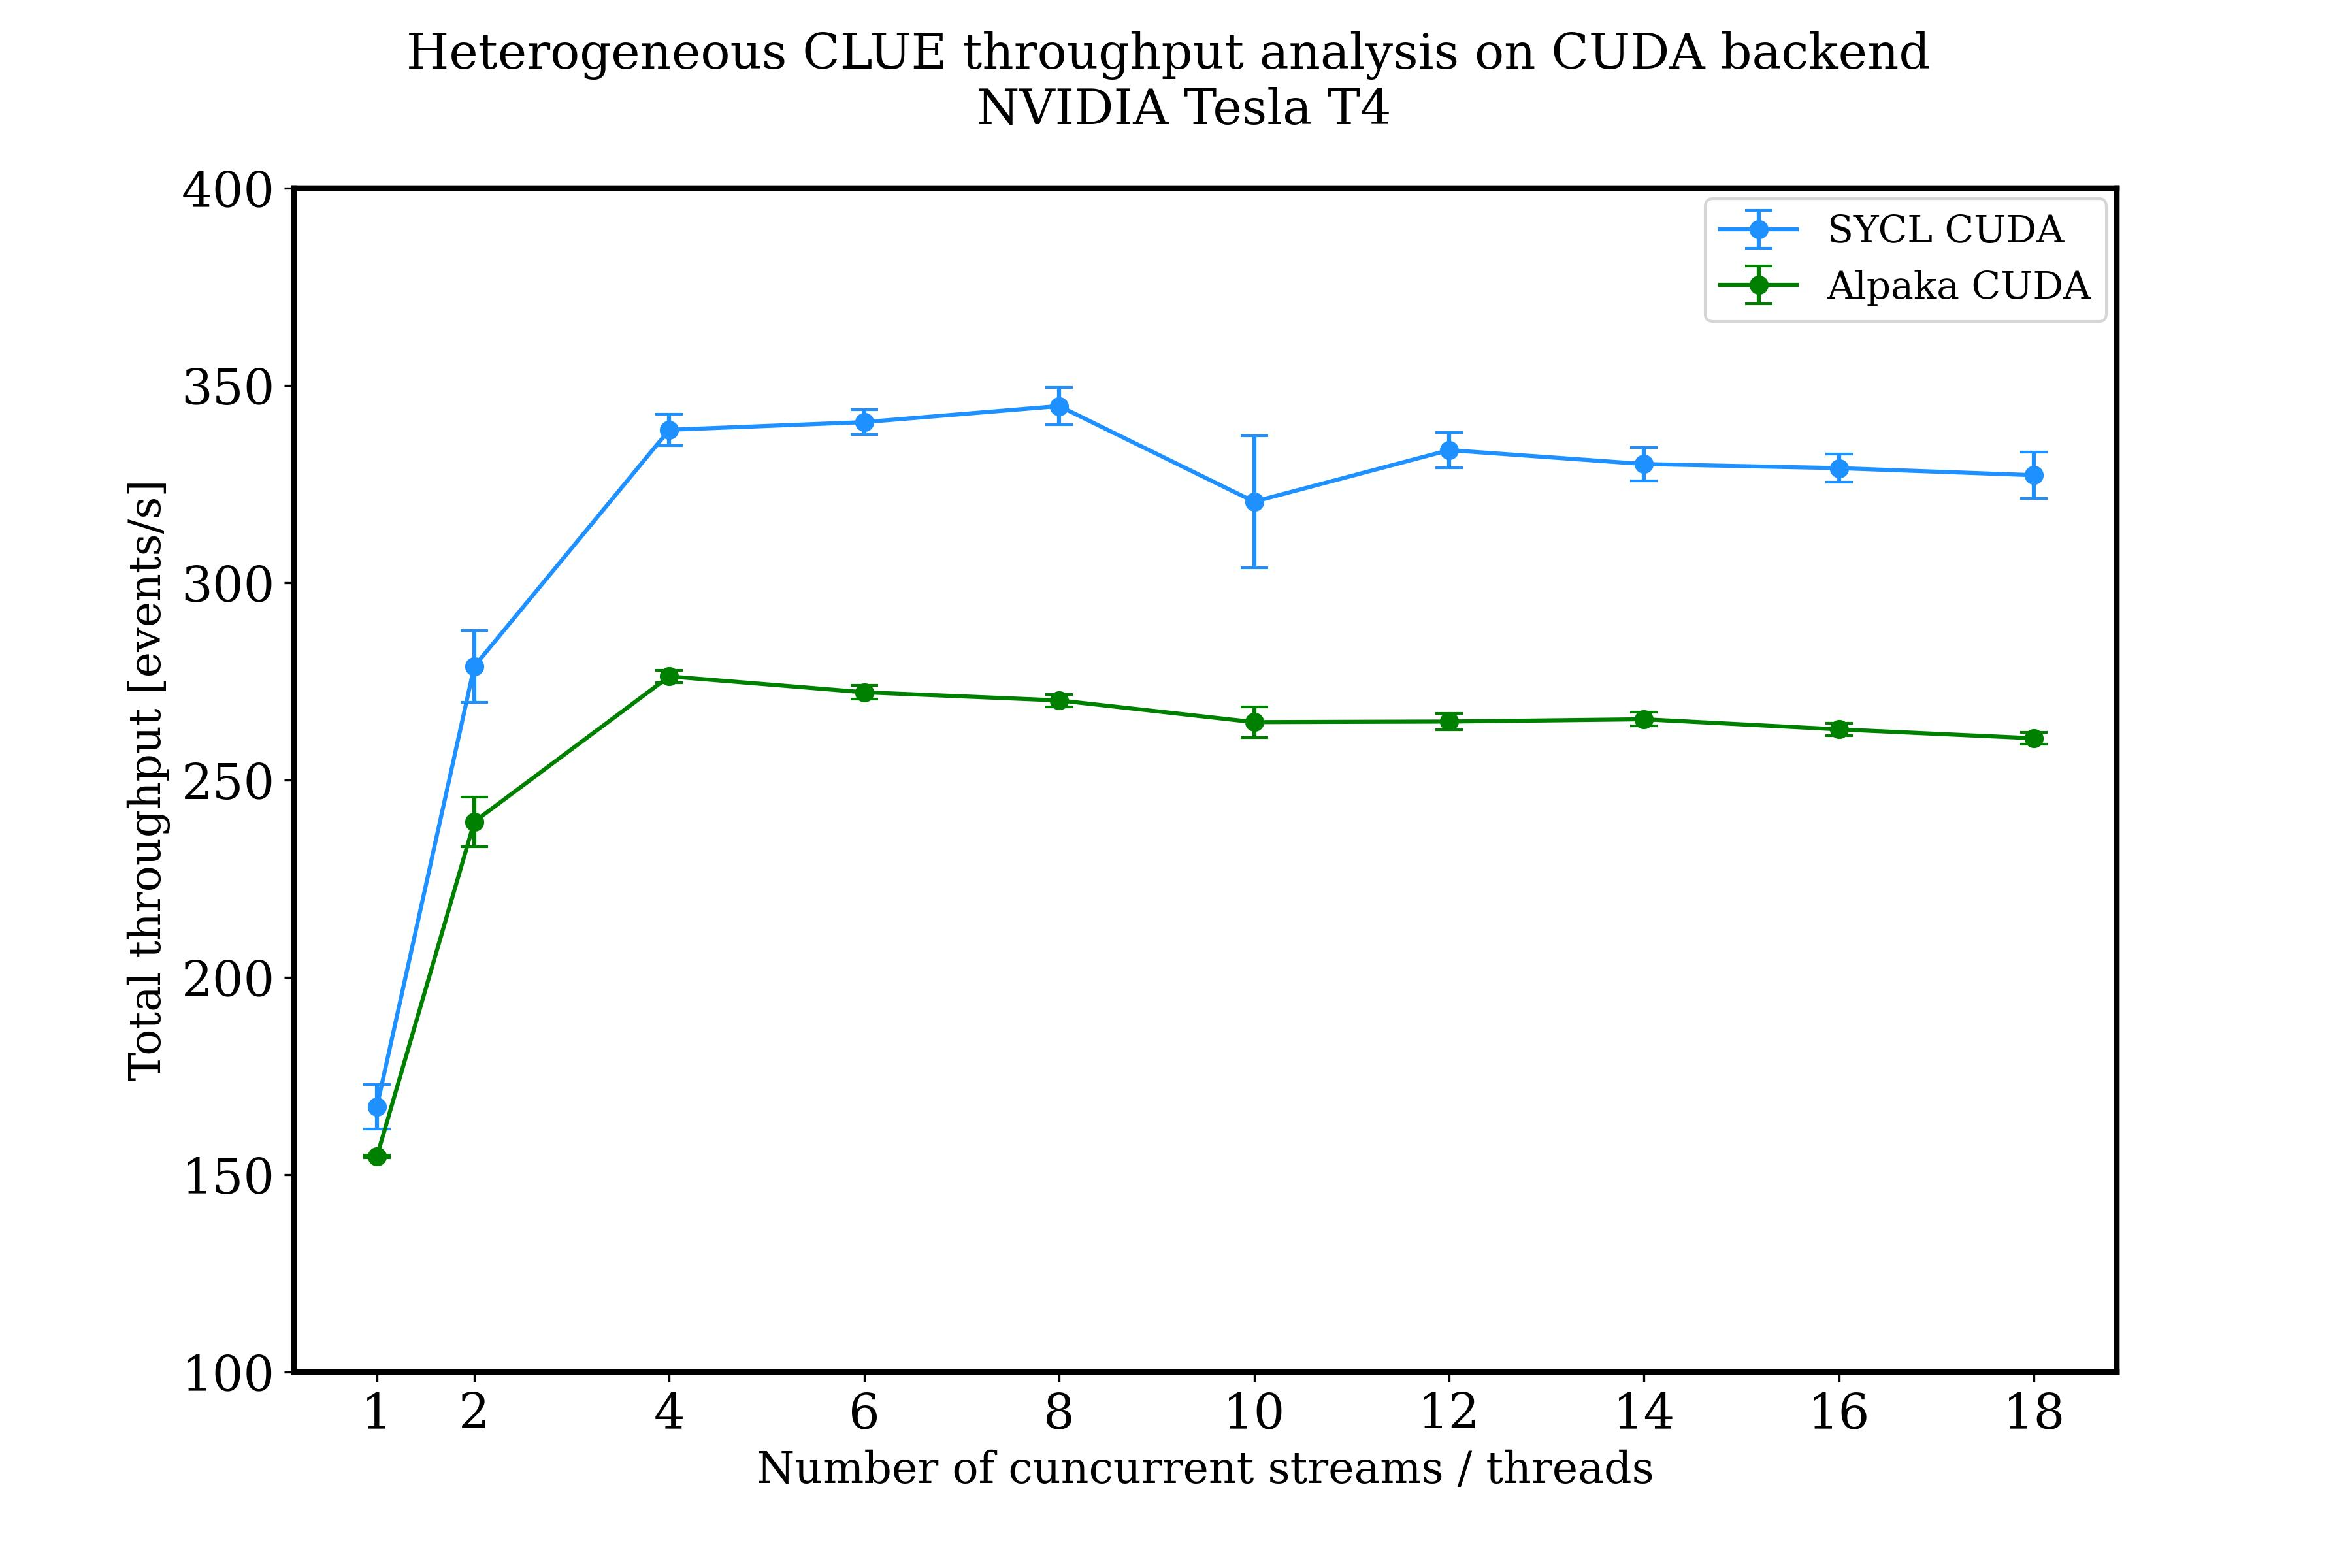
\includegraphics[width=\textwidth]{media/hclue_cuda_performance.jpg}
    \caption{Comparison of SYCL and Alpaka heterogeneous CLUE implementations when running on the CUDA backend (higher throughput is better).}
    \label{fig:hclue_cuda_performance}
\end{figure}
\noindent
The difference in performance is harder to explain in this case, but on a general level it seems that, at least for this particular workload and hardware, SYCL has better memory management capabilities than Alpaka and CUDA, thus improving speed when transferring data, allocating or setting memory, and synchronizing streams. One thing to note is that an increasing number of streams can lead to performance degradation and instability, especially on SYCL, which shows its best performance when using 8 threads/streams. A detailed breakdown of the data is presented in Table~\ref{tab:hclue_cuda_performance}.

\begin{table}[H]
    \centering
    \begin{tabular}{|c|r@{}c|r@{}c|r@{}c|}
 \hline
 \multicolumn{7}{|c|}{Total throughput on NVIDIA Tesla T4 (ev/s)} \\
 \hline
 Streams & \multicolumn{2}{c|}{CUDA} & \multicolumn{2}{c|}{Alpaka} & \multicolumn{2}{c|}{SYCL}\\
 \hline
 1 & 154.9 $\pm$&  ~1.7 & 154.6 $\pm$&  ~0.3 & 167 $\pm$&  ~6 \\
 2 & 249 $\pm$&  ~3 & 239 $\pm$&  ~6 & 279 $\pm$&  ~9 \\
 4 & 277.1 $\pm$&  ~0.9 & 277 $\pm$&  ~2 &	339 $\pm$&  ~4 \\
 6 & 273.9 $\pm$&  ~1.5 & 272 $\pm$&  ~2 & 341 $\pm$&  ~3 \\
 8 & 271.1 $\pm$&  ~1.4 & 270 $\pm$&  ~2 & 345 $\pm$&  ~5 \\
 10 & 267.2 $\pm$&  ~1.8 & 265 $\pm$&  ~4 &	321 $\pm$&  ~17 \\
 12 & 266 $\pm$&  ~2 & 265 $\pm$&  ~2 & 334 $\pm$&  ~4 \\
 14 & 265.5 $\pm$&  ~1.9 & 265 $\pm$&  ~2 & 330 $\pm$&  ~4 \\
 16 & 264.8 $\pm$&  ~1,7 & 262 $\pm$&  ~2 &	329 $\pm$&  ~4 \\
 18 & 261.5 $\pm$&  ~1.0 & 261 $\pm$&  ~2 &	327 $\pm$&  ~6 \\
 \hline
\end{tabular}
    \caption{Detailed throughput analysis for the CUDA implementations of heterogeneous CLUE.}
    \label{tab:hclue_cuda_performance}
\end{table}

Finally, throughput analysis on the unreleased Intel GPU cannot be disclosed due to the pre-alpha state of the hardware, which is still under NDA. However, testing on this hardware has been successful in showing that a single SYCL source code can run on CPUs, Intel GPUs, and NVIDIA GPUs. This demonstrates the potential of SYCL as a compatibility layer to ease code maintainability across different backends.

\subsection{Porting considerations}
As discussed, multiple adjustments had to be made in order to transition from CUDA to SYCL. In this context, the compatibility tool developed by Intel has provided help in more than one occasion, but its output cannot yet be trusted in all situations, especially when dealing with more complex projects. In particular, some of the areas in which the tool provides little to no help are:
\begin{itemize}
    \item Porting of more complex projects made up of multiple compilation units;
    \item Error management;
    \item Atomic operations.
\end{itemize}

Regarding the second point, the error management system employed by SYCL is based on throwing and catching exceptions, similar to what is done in plain C++, while CUDA implements its own error management system. Because of this, it is up to the programmer to add the relevant checks to make sure that the SYCL code can handle eventual errors. As far as atomic operations\footnote{In programming, an atomic operation guarantees exclusive access to a particular memory address to the thread that is executing the operation itself.} are concerned, SYCL implementation is still pretty much undocumented and lacks some fundamental CUDA methods. Re-implementing needed methods is possible, but must be done on a case-by-case basis and completely by hand. 

In general, expressing parallelism through SYCL is more difficult than doing the same through CUDA, mostly due to the heterogeneous nature of the SYCL code. The creation of \texttt{nd\_ranges} with the desired dimensions to cover any specific problem is extremely verbose and the methods to obtain the computing capabilities of the device in use are not always helpful in creating an optimized work division. This problem becomes especially evident in complex code that makes extensive use of CUDA warps\footnote{In CUDA, a warp is a collection of 32 threads that execute the same instruction.} which are inherently more difficult to port to other backends. One possible solution is given by utilizing sub-groups in SYCL, though the sub-group dimension is hardware-dependent and needs to be known at compile time in the kernel invocation.

To sum up the porting experience, the compatibility tool proves itself useful in easing the first steps when getting to know SYCL but fails on more complex projects. Everything that is not translated automatically can be ported by hand even if the documentation is not fully developed yet, so the porting involves a lot of tinkering and experimenting to get the desired results. However, the results obtained in the end look promising, but SYCL is not ready for large-scale adoption at this point: both for the ever-changing and evolving nature of the relatively young SYCL standard and the absence of a complete compiler for all the supported backends.